\documentclass[12pt]{report}
\usepackage[utf8]{inputenc}
\usepackage[T1]{fontenc}
\usepackage{graphicx}
\usepackage{booktabs}
\usepackage{array}
\usepackage{enumitem}
\usepackage{float}
\usepackage{caption}
\usepackage{subcaption}
\usepackage{amsmath}
\usepackage{amssymb}
\usepackage{tikz}
\usetikzlibrary{arrows.meta, positioning, calc}
\usepackage{pgfplots}
\pgfplotsset{compat=1.18}
\usepgfplotslibrary{fillbetween}
\usepackage{listings}
\lstset{basicstyle=\ttfamily\footnotesize, breaklines=true, frame=single, showstringspaces=false,
        columns=fullflexible, keepspaces=true, aboveskip=6pt, belowskip=4pt}
% Placeholder box for app screenshots pending capture (D8). #1 = height, #2 = label.
\newcommand{\screenshotplaceholder}[2]{\fbox{\begin{minipage}[c][#1][c]{0.82\linewidth}\centering\itshape\footnotesize Screenshot placeholder\\[3pt]#2\end{minipage}}}
\usepackage{hyperref}
\usepackage{geometry}
\geometry{a4paper, margin=1in}
\setcounter{secnumdepth}{3} % number sub-subsections (e.g. 2.1.1)

% =====================================================================
% 3rd-Review report (Phase 1, Pillar A). MODULAR layout (D12): front matter
% and bibliography live here; each chapter is its own file under chapters/
% (edit those). Decisions in DECISIONS.md (D1-D12). Voice per
% college/mydeliverables/REPORT_WRITING_GUIDE.md. Figures per
% TIKZ_DIAGRAM_GUIDE.md. Build in /tmp (repo mount is create-only).
% =====================================================================

\begin{document}

\begin{center}

\includegraphics[width=5cm]{PESU-new-logo.png} \\[0.5cm]
\textbf{\Large Dissertation on}\\[1cm]
\textbf{\Huge ``Adaptive Study Planning for\\ Self-Directed Learners''}\\[1cm]

Submitted in partial fulfilment of the requirements for the award of degree of\\[1cm]
\textbf{\Large Master of Technology in}\\[1cm]
\textbf{\Large Data Science and Artificial Intelligence}\\[1cm]
\textbf{UE20CS971 Project Phase - 1}\\[1cm]

\textbf{Submitted by:}\\
\textbf{Rohit Saji}\\
\textbf{PES2PGE24DS201}\\[1cm]

Under the guidance of\\
Prof. Ramesh Prakash Guledgudd\\
PES University\\[1cm]

May -- October 2026\\[1cm]

M.TECH IN DATA SCIENCE AND ARTIFICIAL INTELLIGENCE\\
FACULTY OF ENGINEERING\\
PES UNIVERSITY\\[1cm]
(Established under Karnataka Act No. 16 of 2013)\\
Electronic City, Hosur Road, Bengaluru -- 560 100, Karnataka, India
\end{center}

\newpage

\section*{Certificate}
This is to certify that the dissertation entitled ``Adaptive Study Planning for Self-Directed Learners'' is a bonafide work carried out by \textbf{Rohit Saji (PES2PGE24DS201)} in partial fulfilment for the completion of Project Phase - 1 in the Program of Study -- Master of Technology in Data Science and Artificial Intelligence under the rules and regulations of PES University, Bengaluru.

\vspace{2cm}
\begin{flushright}
Prof. Ramesh Prakash Guledgudd\\
PES University
\end{flushright}

\newpage

\section*{Declaration}
I hereby declare that the Project Phase - 1 entitled ``Adaptive Study Planning for Self-Directed Learners'' has been carried out under the guidance of Prof. Ramesh Prakash Guledgudd, and submitted in partial fulfilment of the course requirements for the award of the degree of Master of Technology in Data Science and Artificial Intelligence of PES University, Bengaluru, during the academic semester May -- October 2026.

\newpage

\section*{Acknowledgement}
I would like to express my gratitude to my guide for continuous guidance and support throughout this project, and to the project coordinators for their help. I thank the Chairperson and faculty of the Department, PES University, for their support, and the university leadership for the opportunities provided. Finally, I extend heartfelt thanks to my family and friends for their constant encouragement.

\newpage

\section*{Abstract}
% Pillar-A, forward narrative, honest (D2/D3/D4/D11). Refined during drafting.
Self-directed learners routinely commit to a fixed study plan and fall behind or move ahead within days, yet the plan does not adapt and the learner has no reliable signal of how far off-track they are. This work develops an adaptive study-planning system for a single self-directed learner and evaluates the algorithms behind it. The system estimates a learner's true study pace from their own session history using hierarchical Bayesian calibration with a shrinkage-regularized context model, detects behavioural shifts in that pace using CUSUM change-point detection, and projects the completion date with a calibrated uncertainty band using Gaussian-process regression, regenerating the plan when the learner's realised pace diverges from the schedule. Each component is compared against established baselines on a literature-grounded synthetic dataset with known ground truth, using held-out evaluation with bootstrap confidence intervals and Holm/Benjamini--Hochberg correction. Phase~I delivers and evaluates this open-loop system and reports the comparison; Phase~II will close the loop with assessment-based verification of genuine learning. The selected models are realised in a working local-first web application.

\newpage
\tableofcontents
\newpage
\listoffigures
\newpage
\listoftables
\newpage

% ---- Chapters (modular; one file each under chapters/) ----
\chapter{Introduction}
This chapter sets out the problem the project addresses and the shape of the work that follows. Section~1.1 states the problem faced by self-directed learners and the motivation for an adaptive study planner. Section~1.2 lists the objectives of Phase~I. Section~1.3 defines the scope of the work across the two project phases. Section~1.4 describes the organization of the remainder of the report.

\section{Problem Statement}
A self-directed learner is a person who works through online courses, examination preparation, or self-study material without an instructor setting the pace. Such a learner typically begins with a fixed plan, of the form ``two hours a day, finish by this date.'' The plan is a one-time estimate. It assumes that the learner will study at the rate they intended and that the material will take as long as they guessed.

Within a few days the plan no longer matches reality. The learner falls behind on some days and moves ahead on others, the estimate of how long each item takes proves wrong, and the fixed plan does not adjust. The learner is left without a trustworthy signal of how far off-track they are or when they will actually finish. The estimate that mattered at the start, the finish date, silently becomes inaccurate while the plan continues to display it as though it were still valid.

Existing tools address only one side of this problem. Time-tracking applications record how long a learner studied but do not plan; static plan generators produce a schedule once and never revise it against the rate the learner actually achieves. Neither learns the learner's realised pace, and neither revises the finish-date estimate as evidence accumulates. The gap this project addresses is the absence of a planner that treats the learner's own logged behaviour as evidence, updates its estimate of their pace as that evidence arrives, and regenerates the plan accordingly.

The difficulty is that the evidence is sparse. A single learner produces only a handful of study sessions before the plan first needs to adapt, so a method that requires large amounts of per-learner data is not usable here. The pace is also not stationary: it shifts when the learner's circumstances change, and a useful system must distinguish a genuine shift from ordinary day-to-day variation before it acts. These two constraints, sparse data and non-stationary behaviour, shape the choice of methods in the chapters that follow.

\section{Objectives}
Phase~I of the project pursues the following objectives.
\begin{enumerate}[noitemsep]
    \item Estimate a learner's true study pace from their own session history using hierarchical Bayesian calibration with a context-aware shrinkage model, so that a usable estimate is available from few sessions.
    \item Detect behavioural shifts in the learner's pace using statistical change-point detection, so that the plan adapts to a genuine change rather than to noise.
    \item Project the learner's completion date with a calibrated uncertainty band, rather than a single point, using Gaussian-process regression over the accumulated progress.
    \item Regenerate the study schedule from the learner's realised capacity when the projected finish date diverges from the deadline.
    \item Evaluate each component against established baselines on a synthetic dataset with known ground truth, using held-out evaluation with bootstrap confidence intervals and multiple-comparison correction.
    \item Realise the selected models in a working, local-first web application for a single self-directed learner.
\end{enumerate}

\section{Scope of the Project}
The work is delivered across two phases. \textbf{Phase~I}, reported here, builds and evaluates the open-loop system. Its components are pace calibration, change detection, completion projection, and capacity-based schedule regeneration. Each is compared offline against baselines on synthetic data with known ground truth, and the selected models are realised in the application. The target user is the individual self-directed learner.

\textbf{Phase~II} will close the loop and add assessment-based verification of genuine learning, so that the pace signal driving the plan is checked against evidence that studying produced learning rather than against self-reported time alone. Phase~II will also validate the system longitudinally on a single learner's real logged sessions. Multi-user, institutional, and instructor-mediated settings are out of scope for both phases.

\section{Organization of the Report}
The remainder of the report is organized as follows. Chapter~2 surveys the research the project draws on, grouped by technique, and states the gaps it addresses. Chapter~3 specifies the hardware, software, and functional requirements of the system. Chapter~4 describes the proposed methodology: the candidate models for each component, the offline comparison methodology, the system design and how it evolved during development, and the resulting architecture. Chapter~5 gives the implementation details, including the datasets and their sources and the realised application. Chapter~6 presents and discusses the comparison results. Chapter~7 concludes Phase~I and sets out the work planned for Phase~II.

\chapter{Literature Survey}
This chapter surveys the techniques the project draws on, organized by the components of the adaptive planner and the analytics that motivate them. Section~2.1 reviews learner pace modelling and Bayesian calibration. Section~2.2 covers behavioural-change detection. Section~2.3 surveys progress prediction with Gaussian processes. Section~2.4 reviews adaptive scheduling and study-plan generation. Section~2.5 covers self-regulated-learning analytics. Section~2.6 describes the methodology used to source and screen the surveyed literature. Section~2.7 summarizes the approaches, states their limitations for this project, and positions the proposed solution.

\section{Learner Pace Modelling and Bayesian Calibration}
Estimating how fast a learner truly works, from limited per-learner data, is the foundation of the planner. Chen et al.~\cite{chen2024} present a hierarchical Bayesian model of adaptive teaching and validate it through two online behavioural experiments with 312 adults, showing that hierarchical priors capture learner-to-learner variability without overfitting to sparse data. This is the statistical justification for estimating a single learner's pace from few sessions. The model targets a teacher's choice of examples rather than the planned-versus-actual pace this project estimates, so it supplies the prior structure but not the quantity to be calibrated.

The pace signal itself is simple to state. For a session the pace ratio is $r_t = a_t / p_t$, the ratio of active minutes $a_t$ to planned minutes $p_t$, modelled as $r_t \sim \mathcal{N}(\mu,\sigma^2)$ with a prior $\mu \sim \mathcal{N}(\mu_0,\tau_0^2)$ centred at $\mu_0=1$ (the learner works at the planned rate). With $n$ observed sessions the conjugate posterior is Gaussian,
\begin{equation}
p(\mu \mid r_{1:n}) = \mathcal{N}(\mu_n,\tau_n^2), \qquad
\tau_n^2 = \Big(\tfrac{1}{\tau_0^2}+\tfrac{n}{\sigma^2}\Big)^{-1}, \qquad
\mu_n = \tau_n^2\Big(\tfrac{\mu_0}{\tau_0^2}+\tfrac{1}{\sigma^2}\sum_{t=1}^{n} r_t\Big).
\label{eq:bayes-update}
\end{equation}
When $n$ is small the posterior stays close to the prior, which is what lets a usable estimate exist from a handful of sessions; as $n$ grows the data term dominates and the estimate tightens around the learner's realised rate, as illustrated in Figure~\ref{fig:bayes-update}.

\begin{figure}[htbp]
\centering
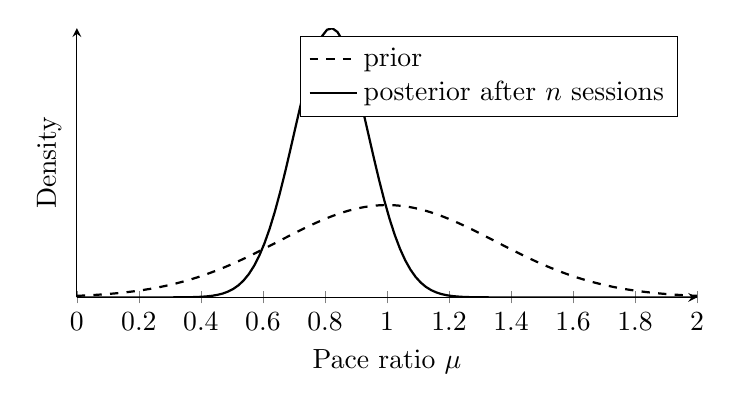
\begin{tikzpicture}
\begin{axis}[width=0.78\linewidth, height=5cm, xlabel={Pace ratio $\mu$}, ylabel={Density}, domain=0:2, samples=120, ymin=0, xmin=0, xmax=2, axis lines=left, ytick=\empty, legend pos=north east, legend cell align=left]
\addplot[thick, dashed]{exp(-(x-1)^2/(2*0.35^2))/(0.35*sqrt(2*pi))};
\addlegendentry{prior}
\addplot[thick]{exp(-(x-0.82)^2/(2*0.12^2))/(0.12*sqrt(2*pi))};
\addlegendentry{posterior after $n$ sessions}
\end{axis}
\end{tikzpicture}
\caption{Schematic illustration of Bayesian pace calibration by Equation~\eqref{eq:bayes-update}: a broad prior over the pace ratio (dashed) tightens to a narrower posterior (solid) as session evidence accumulates. The values shown are illustrative, not measured.}
\label{fig:bayes-update}
\end{figure}

Zanellati et al.~\cite{zanellati2024} review hybrid knowledge-tracing models in a taxonomy of approaches that combine Bayesian posteriors with machine learning, and conclude that hybrid models consistently outperform either pure Bayesian Knowledge Tracing or pure deep learning. Zambrano et al.~\cite{zambrano2024} analyse algorithmic bias in Bayesian Knowledge Tracing at scale and report that performance is essentially equal across demographic groups, which supports the reliable use of Bayesian-family models across diverse learners. Mai et al.~\cite{mai2025} couple deep temporal modelling with a probabilistic layer in a Transformer--Bayesian hybrid that recovers interpretable, calibrated knowledge estimates, reinforcing that a hybrid Bayesian design keeps transparency without sacrificing predictive accuracy. These works establish Bayesian calibration as sound for learner modelling, but they address correctness prediction rather than the planned-versus-actual pace estimation this project requires.

\section{Behavioural-Change Detection}
A learner's pace is not stationary, and detecting when it shifts is what makes timely replanning possible. Saqr et al.~\cite{saqr2026} apply critical-slowing-down indicators in an idiographic analysis of 1.67~million practice attempts from 9{,}401 students and find that 88.2\% of disengaging learners exhibit detectable warning signals beforehand, which is strong evidence that per-learner behavioural shifts are recoverable from trace data. Qiao et al.~\cite{qiao2026} provide a PRISMA systematic review of statistical-process-control methods and document the rationale for CUSUM and EWMA control charts and their machine-learning-enhanced variants, though the reviewed applications target manufacturing rather than education.

The cumulative-sum chart is the detector this project builds on. A one-sided chart tracks the running deviation of the pace signal $x_t$ from its in-control mean $\mu_0$,
\begin{equation}
S_0 = 0, \qquad S_t = \max\!\big(0,\; S_{t-1} + (x_t-\mu_0) - k\big), \qquad \text{alarm if } S_t > h,
\label{eq:cusum}
\end{equation}
where the slack $k$ absorbs ordinary day-to-day variation and $h$ is the decision threshold~\cite{qiao2026}. The statistic stays near zero while the pace is stable and accumulates once a genuine shift occurs, raising an alarm when it crosses $h$, as illustrated in Figure~\ref{fig:cusum}.

\begin{figure}[htbp]
\centering
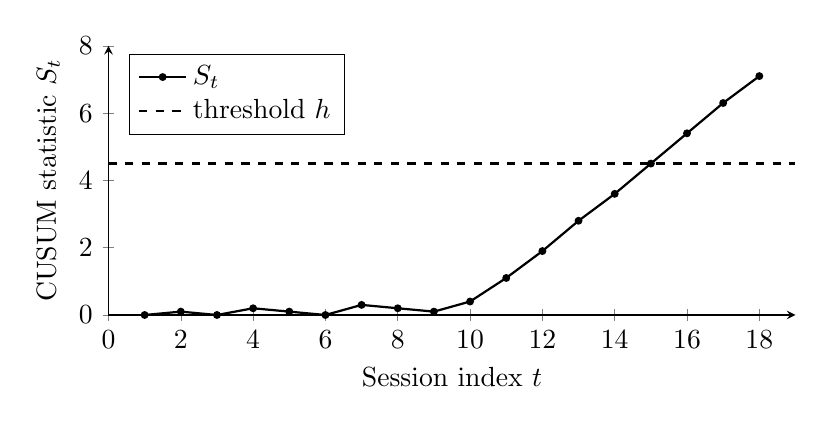
\begin{tikzpicture}
\begin{axis}[width=0.85\linewidth, height=5cm, xlabel={Session index $t$}, ylabel={CUSUM statistic $S_t$}, xmin=0, xmax=19, ymin=0, ymax=8, axis lines=left, legend pos=north west, legend cell align=left]
\addplot[thick, mark=*, mark size=1pt] coordinates {(1,0)(2,0.1)(3,0)(4,0.2)(5,0.1)(6,0)(7,0.3)(8,0.2)(9,0.1)(10,0.4)(11,1.1)(12,1.9)(13,2.8)(14,3.6)(15,4.5)(16,5.4)(17,6.3)(18,7.1)};
\addlegendentry{$S_t$}
\addplot[thick, dashed, domain=0:19]{4.5};
\addlegendentry{threshold $h$}
\end{axis}
\end{tikzpicture}
\caption{Schematic illustration of one-sided CUSUM detection by Equation~\eqref{eq:cusum}: the statistic stays near zero while the pace is stable and accumulates after a shift near $t=10$, raising an alarm when it crosses the threshold $h$. The values shown are illustrative.}
\label{fig:cusum}
\end{figure}

Boca de Giuli et al.~\cite{boca2024} combine control charts with continual learning to separate endogenous system shifts from one-time exogenous disruptions, a distinction that maps directly onto the need to recalibrate on genuine pace change while ignoring a one-off disruption. Cheng et al.~\cite{cheng2024} model behavioural change directly from heterogeneous student records for early at-risk prediction, deliberately retaining qualitative information that pure feature extraction discards. The limitation shared across these methods is that they detect a shift but prescribe no corrective action, which is the step this project adds by feeding the detected shift into replanning.

\section{Progress Prediction with Gaussian Processes}
Projecting a completion date with a calibrated uncertainty band, rather than a single number, is what makes a projection trustworthy. P\'erez-Suay et al.~\cite{perezsuay2024} apply Gaussian-process (GP) regression with an automatic-relevance-determination kernel to learning-management-system logs and achieve a correlation of $R = 0.89$ for predicting student marks, with interpretable feature weighting. Chen and Yao~\cite{chenyao2025} combine black-hole optimisation for feature selection with a weighted GP-regression ensemble, reporting a root-mean-square error of 0.95 and a mean absolute error of 0.81, and show that GP predictions degrade gracefully as data becomes scarce.

A Gaussian process places a prior over progress curves and conditions it on the observed points. For a test time $x_*$ the predictive distribution is Gaussian, with mean and variance
\begin{equation}
\bar{f}_* = \mathbf{k}_*^{\top}(K+\sigma_n^2 I)^{-1}\mathbf{y}, \qquad
\mathbb{V}[f_*] = k(x_*,x_*) - \mathbf{k}_*^{\top}(K+\sigma_n^2 I)^{-1}\mathbf{k}_*,
\label{eq:gp-pred}
\end{equation}
under a squared-exponential kernel with signal variance $\sigma_f^2$ and length scale $\ell$,
\begin{equation}
k(x,x') = \sigma_f^2 \exp\!\Big(-\tfrac{(x-x')^2}{2\ell^2}\Big).
\label{eq:gp-kernel}
\end{equation}
The predictive variance in Equation~\eqref{eq:gp-pred} is what supplies a calibrated band around the projected finish date, rather than a single point, as illustrated in Figure~\ref{fig:gp-burnup}.

\begin{figure}[htbp]
\centering
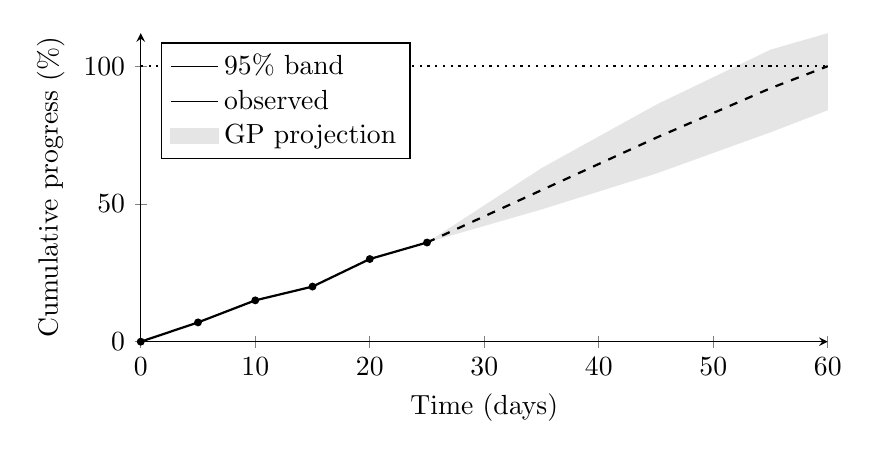
\begin{tikzpicture}
\begin{axis}[width=0.85\linewidth, height=5.5cm, xlabel={Time (days)}, ylabel={Cumulative progress (\%)}, xmin=0, xmax=60, ymin=0, ymax=112, axis lines=left, legend pos=north west, legend cell align=left]
\addplot[name path=up, draw=none] coordinates {(25,36)(35,63)(45,86)(55,106)(60,112)};
\addplot[name path=lo, draw=none] coordinates {(25,36)(35,48)(45,61)(55,76)(60,84)};
\addplot[gray!20] fill between[of=up and lo];
\addlegendentry{95\% band}
\addplot[thick, mark=*, mark size=1pt] coordinates {(0,0)(5,7)(10,15)(15,20)(20,30)(25,36)};
\addlegendentry{observed}
\addplot[thick, dashed] coordinates {(25,36)(35,55)(45,74)(55,92)(60,100)};
\addlegendentry{GP projection}
\addplot[thick, dotted, domain=0:60]{100};
\end{axis}
\end{tikzpicture}
\caption{Schematic illustration of a Gaussian-process burn-up projection: observed cumulative progress (solid) is extrapolated to completion (dashed) with a 95\% band that widens with the horizon; the dotted line marks 100\% completion. The values shown are illustrative.}
\label{fig:gp-burnup}
\end{figure}

Lin et al.~\cite{lin2024} introduce a latent Kronecker structure to scale GPs for learning-curve prediction, matching Transformer performance while retaining calibrated uncertainty. Beyond regression, Huang and Wang~\cite{huang2025} use Gaussian-process classification with a meta-heuristic hyper-parameter search to predict student performance bands, and Kayande and Kukreja~\cite{kayande2025} report an integrated multi-modal machine-learning framework for engagement and dropout prediction on educational data. These works validate GP methods on educational data, but they apply the model cross-sectionally to a final outcome rather than to the longitudinal burn-up projection, with a running finish-date estimate, that this project needs.

\section{Adaptive Scheduling and Study-Plan Generation}
The system must turn its estimates into a concrete, regenerated schedule. Islam et al.~\cite{islam2024} couple an artificial neural network for grade prediction, at an accuracy of about 0.73, with dynamic programming for optimal schedule allocation, establishing the predict-then-optimize architecture this project takes as its Pillar-A base paper. The two stages are shown in Figure~\ref{fig:predict-optimize}: a predictive model estimates the learner's pace, and an optimizer turns that estimate into a schedule.

\begin{figure}[htbp]
\centering
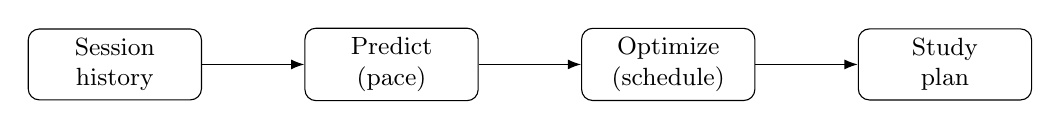
\begin{tikzpicture}[node distance=6mm and 13mm, box/.style={draw, rounded corners, minimum height=9mm, minimum width=22mm, align=center, font=\small}, >=Latex]
\node[box] (hist) {Session\\history};
\node[box, right=of hist] (predict) {Predict\\(pace)};
\node[box, right=of predict] (opt) {Optimize\\(schedule)};
\node[box, right=of opt] (plan) {Study\\plan};
\draw[->] (hist) -- (predict);
\draw[->] (predict) -- (opt);
\draw[->] (opt) -- (plan);
\end{tikzpicture}
\caption{The predict-then-optimize architecture~\cite{islam2024} this project adopts and extends: a predictive model estimates the learner's pace, and an optimizer turns the estimate into a schedule.}
\label{fig:predict-optimize}
\end{figure}

The optimize step solves a scheduling problem by dynamic programming. Writing $V(t,\rho)$ for the best achievable cost from day $t$ onward with remaining work $\rho$, the schedule follows a recurrence of the form
\begin{equation}
V(t,\rho) = \min_{0 \le a \le c_t}\ \big[\, \ell(a) + V(t+1,\ \rho - a)\,\big],
\label{eq:dp}
\end{equation}
where $a$ is the study time allocated on day $t$, $c_t$ is that day's capacity, and $\ell$ penalises deadline drift~\cite{islam2024}. Fabregar and Amorado~\cite{fabregar2025} generate expert-quality study plans in 0.32~seconds using a greedy algorithm with prerequisite-constraint satisfaction, which demonstrates fast constraint-based, prerequisite-aware scheduling. Pagano et al.~\cite{pagano2026} report a controlled study of 2{,}064 students in which adaptive learning paths produce substantial efficiency gains over static ones, giving both large-scale evidence that adaptation helps and a template for an adaptive-versus-static evaluation design. Liu et al.~\cite{liu2025} integrate a domain knowledge graph with AI-driven sequencing to construct personalised learning paths that respect concept prerequisites. The limitation across these works is that the generated plan is solved once and does not adapt to the pace the learner actually achieves, which is the feedback this project adds.

\section{Self-Regulated-Learning Analytics}
Self-regulated-learning (SRL) analytics grounds the choice of metrics for a planner that reports back to the learner. Alhazbi et al.~\cite{alhazbi2024} review 25 empirical studies on measuring SRL from trace data and find that most validated indicators relate to time-management skills, which grounds this project's use of schedule adherence and regularity as its behavioural metrics. de Barba et al.~\cite{debarba2025} develop and validate an SRL learning-analytics rubric that maps validated SRL scales onto learning-management-system indicators in a scalable, explainable way.

Uzun et al.~\cite{uzun2025} show that a learner's engagement with analytics feedback is associated with both SRL competence and course performance, which motivates the feedback-oriented design of this project's dashboards. Butt et al.~\cite{butt2025} apply a hybrid machine-learning and rough-set model to identify at-risk learners and trigger personalised interventions. These works supply validated, trace-based indicators of self-regulation, but they stop at the feedback step shown in Figure~\ref{fig:srl-loop}, and none feeds the SRL signal back into an adaptive plan.

\begin{figure}[htbp]
\centering
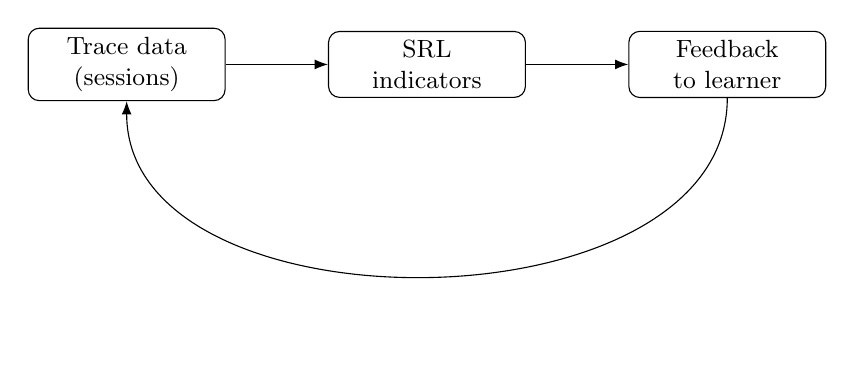
\begin{tikzpicture}[node distance=7mm and 13mm, box/.style={draw, rounded corners, minimum height=8mm, minimum width=25mm, align=center, font=\small}, >=Latex]
\node[box] (trace) {Trace data\\(sessions)};
\node[box, right=of trace] (ind) {SRL\\indicators};
\node[box, right=of ind] (fb) {Feedback\\to learner};
\draw[->] (trace) -- (ind);
\draw[->] (ind) -- (fb);
\draw[->] (fb.south) to[out=-90, in=-90] (trace.south);
\end{tikzpicture}
\caption{The self-regulated-learning analytics loop the reviewed work supports: trace data yields validated indicators that are fed back to the learner. The reviewed systems stop at feedback; this project extends the loop by feeding the signal into replanning.}
\label{fig:srl-loop}
\end{figure}

\section{Methodology for Sourcing the Surveyed Models}
The literature above was assembled through a repeatable screening pipeline rather than by ad-hoc reading, so that the coverage of each theme is defensible. A raw candidate list of 107 Pillar-A digital object identifiers was collected from database and citation searches. Each candidate was enriched with metadata from CrossRef, OpenAlex, and arXiv, and scored against twelve weighted keyword clusters aligned with the project's components, including Bayesian calibration, change-point detection, Gaussian-process regression, adaptive scheduling, and self-regulated learning. The score thresholded each paper into a strong, good, partial, or weak fit.

The score was treated as advisory rather than decisive. Final selection favoured topical coverage across sub-themes over raw score: one representative work was kept per sub-theme, and higher-scoring but redundant papers were dropped, while a lower-scoring paper was retained when it was the best available fit for a specific narrative role. The screening also rejected keyword false positives, where a paper matched a cluster keyword but was topically unrelated. This curation reduced the raw list to the set of works surveyed in this chapter.

\section{Summary of Approaches}
Table~\ref{tab:litsummary} summarizes the approach families across the components with their strengths and the limitations that motivate this work. The recurring pattern is that each technique is strong in isolation but disconnected from the others: none forms a closed loop from realised pace back to the plan.

\begin{table}[htbp]
\centering
\footnotesize
\caption{Summary of Pillar-A approach families, with strengths and limitations for this project.}
\label{tab:litsummary}
\begin{tabular}{p{3.0cm} p{4.2cm} p{4.2cm}}
\toprule
\textbf{Approach family} & \textbf{Strengths} & \textbf{Limitations for this project} \\
\midrule
Bayesian calibration~\cite{chen2024,zanellati2024,zambrano2024,mai2025} & Works with sparse, per-learner data; interpretable; fair across groups & Targets correctness, not planned-versus-actual pace \\
Change-point detection~\cite{saqr2026,qiao2026,boca2024,cheng2024} & Detects behavioural shifts early; well-founded in statistical process control & Detects only; prescribes no corrective replanning \\
Gaussian-process projection~\cite{perezsuay2024,chenyao2025,lin2024,huang2025,kayande2025} & Calibrated uncertainty; degrades gracefully with little data & Applied cross-sectionally, not to longitudinal burn-up \\
Adaptive scheduling~\cite{islam2024,fabregar2025,pagano2026,liu2025} & Fast, prerequisite-aware; adaptation shown to help & Generated plan is static; no feedback from realised pace \\
SRL analytics~\cite{alhazbi2024,debarba2025,uzun2025,butt2025} & Validated trace-based indicators of self-regulation & Measures behaviour; not tied to adaptive replanning \\
\bottomrule
\end{tabular}
\end{table}

The limitations that motivate this project follow from the table. First, calibration, change detection, projection, and scheduling are each studied in isolation, and no reviewed system integrates them into a single connected loop. Second, behavioural monitoring detects shifts but prescribes no corrective replanning, and the scheduling work is static and does not adapt to realised pace. Third, the Gaussian-process work is cross-sectional, so calibrated learning-curve projection is not applied to ongoing self-directed study. Fourth, self-regulated-learning analytics supplies validated indicators but stops at measurement, without feeding the signal back into the plan.

This project addresses these gaps by extending the predict-then-optimize architecture~\cite{islam2024} into an adaptive loop for a single self-directed learner. It combines hierarchical Bayesian pace calibration with a context-aware shrinkage model~\cite{chen2024}, change-point detection of behavioural shifts surfaced as a recalibration prompt~\cite{saqr2026,qiao2026}, Gaussian-process progress projection with a calibrated uncertainty band~\cite{perezsuay2024}, and capacity-based schedule regeneration~\cite{fabregar2025}, evaluated with the adaptive-versus-static paradigm~\cite{pagano2026} and self-regulated-learning metrics~\cite{alhazbi2024}. Phase~II will extend this open-loop system with assessment-based verification of genuine learning, so that the pace signal driving the plan is checked against evidence of learning rather than self-reported time alone.

\chapter{System Requirements Specification}
This chapter specifies the requirements of the Phase-I system. Section~3.1 states the hardware environment. Section~3.2 states the software environment. Section~3.3 lists the functional requirements as numbered items, and Section~3.4 lists the non-functional requirements.

\section{Hardware Requirements}
The system is designed to run on commodity hardware. A single learner produces a small volume of data, and every model trains and runs on a CPU, so no dedicated graphics processor is required. Table~\ref{tab:hardware} lists the hardware environment.

\begin{table}[htbp]
\centering
\caption{Hardware environment.}
\label{tab:hardware}
\begin{tabular}{p{4.2cm} p{8.0cm}}
\toprule
\textbf{Component} & \textbf{Requirement} \\
\midrule
Processor & Any modern x86-64 or ARM CPU; no GPU required \\
Memory & 8~GB RAM or higher \\
Storage & A few gigabytes for the container image and local data \\
Container runtime & Docker (via Colima on macOS) to run the intelligence service \\
Client device & Any device with a modern web browser \\
\bottomrule
\end{tabular}
\end{table}

\section{Software Requirements}
The system is organised into three tiers: a local-first browser client, a Python intelligence service that hosts the heavier statistical models, and an offline research pipeline used to compare and select those models. Supabase provides authentication, the event database, and object storage that link the client and the service. Table~\ref{tab:software} lists the software environment by tier.

\begin{table}[htbp]
\centering
\caption{Software environment by tier.}
\label{tab:software}
\begin{tabular}{p{3.6cm} p{8.6cm}}
\toprule
\textbf{Tier} & \textbf{Technologies} \\
\midrule
Client (single-page app) & React~19, Vite, TypeScript, Dexie over IndexedDB for local-first storage, date-fns \\
Intelligence service & Python~3.12, FastAPI, Uvicorn, NumPy and SciPy, PyJWT; packaged with Docker \\
Backend services & Supabase: authentication, a PostgreSQL event database, and object storage \\
Offline research pipeline & Python (uv workspace), NumPy, with pytest and ruff for testing and linting \\
Tooling and deployment & pnpm workspace, Vitest and Playwright for testing, Vercel for hosting \\
\bottomrule
\end{tabular}
\end{table}

\section{Functional Requirements}
The functional requirements state what the Phase-I system does.
\begin{enumerate}[label=\textbf{FR-\arabic*},noitemsep,leftmargin=*]
    \item The system shall let a learner define a study plan from a set of materials, a deadline, and a weekly study capacity.
    \item The system shall log study sessions, both from an in-application timer and from manual entry of a past session.
    \item The system shall estimate the learner's pace from the logged sessions using hierarchical Bayesian calibration.
    \item The system shall detect a shift in the learner's pace and surface a recalibration prompt for the learner to act on.
    \item The system shall project the completion date with a calibrated uncertainty band rather than a single date.
    \item The system shall regenerate the schedule from the learner's realised capacity when the learner chooses to replan.
    \item The system shall present the learner's progress, including the burn-up curve, streak, and schedule adherence.
    \item The system shall persist all data on the device and synchronize it to the cloud when a connection is available.
\end{enumerate}

\section{Non-Functional Requirements}
The non-functional requirements state the qualities the system must exhibit.
\begin{enumerate}[label=\textbf{NFR-\arabic*},noitemsep,leftmargin=*]
    \item \textbf{Offline-first operation.} The core logging loop shall function without network connectivity, and analytical results shall be cached locally for reuse.
    \item \textbf{Commodity scale.} The system shall serve the individual-learner workload on commodity hardware without specialised accelerators.
    \item \textbf{Per-learner isolation.} Each learner's data shall be isolated, using a per-user local database and row-level security in the cloud database.
    \item \textbf{Authenticated services.} Requests to the intelligence service shall carry a signed token that is verified against the identity provider before any model runs.
    \item \textbf{Responsiveness.} Calibration and projection results shall return within a few seconds, with a fallback to the last cached result when the service is unreachable.
    \item \textbf{Behavioural alignment.} Where an algorithm exists in both the client and the service, the two implementations shall be kept behaviourally aligned so that results do not depend on which one runs.
\end{enumerate}

\chapter{Proposed Methodology}
This chapter describes the methodology of the Phase-I system. Section~4.1 presents the adaptive planning loop that ties the four components together. Section~4.2 states the candidate models considered for each component and the model selected for the delivered system. Section~4.3 describes the offline comparison methodology used to make that selection. Section~4.4 records how the system design evolved during development, from a predict-then-optimize scheduler to a capacity-based booking model. Section~4.5 describes the resulting system architecture and the split between client-side and server-side computation.

\section{The Adaptive Planning Loop}
The planner is organised as an open loop over the learner's own logged sessions. A session is logged, the learner's pace is recalibrated from the accumulated history, the pace series is checked for a behavioural shift, the completion date is re-projected, and the schedule is regenerated when the projection diverges from the deadline. The loop is deliberately open rather than automatic: a detected shift raises a recalibration prompt, and the learner decides whether to replan. This keeps the learner in control of a plan that is theirs, and it avoids acting on a shift that the learner knows to be a one-off. Figure~\ref{fig:loop} shows the four components and the signal that passes between them.

\begin{figure}[htbp]
\centering
\resizebox{\linewidth}{!}{%
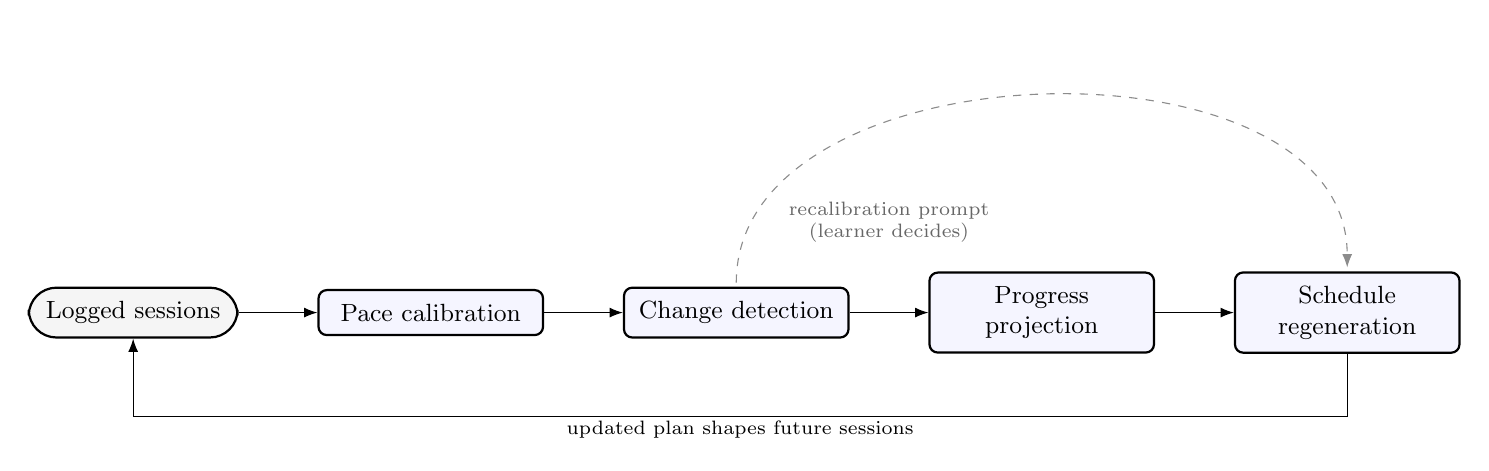
\begin{tikzpicture}[node distance=6mm and 10mm, font=\small, >=Latex,
  lstep/.style={draw, rounded corners=3pt, line width=0.8pt, align=center, inner sep=5pt, text width=2.5cm, fill=blue!4},
  io/.style={draw, rounded corners=10pt, line width=0.8pt, align=center, inner sep=5pt, text width=2.3cm, fill=black!4}]
\node[io] (S) {Logged sessions};
\node[lstep, right=of S] (C) {Pace calibration};
\node[lstep, right=of C] (D) {Change detection};
\node[lstep, right=of D] (P) {Progress projection};
\node[lstep, right=of P] (R) {Schedule regeneration};
\draw[->] (S) -- (C);
\draw[->] (C) -- (D);
\draw[->] (D) -- (P);
\draw[->] (P) -- (R);
\draw[->] (R.south) -- ++(0,-0.8) -| node[pos=0.25, below, font=\scriptsize, fill=white, inner sep=1.5pt]{updated plan shapes future sessions} (S.south);
\node[font=\scriptsize, text=black!60, align=center] at ($(D)!0.5!(P)+(0,1.15)$) {recalibration prompt\\(learner decides)};
\draw[->, dashed, draw=black!45] ($(D.north)+(0,0.05)$) to[out=90,in=90] ($(R.north)+(0,0.05)$);
\end{tikzpicture}%
}
\caption{The open adaptive loop. Logged sessions drive pace calibration, change detection, and progress projection; a detected shift raises a recalibration prompt, and the learner decides whether to regenerate the schedule, which in turn shapes future sessions.}
\label{fig:loop}
\end{figure}

\section{Candidate Models and Selected Approach}
Each component was chosen by comparing candidate models offline rather than by assumption. This section states the candidates and the selected model; Section~4.3 describes how the comparison was run. Table~\ref{tab:candidates} summarises the choices.

\subsection{Pace Calibration}
The calibration candidates were a simple moving average of the pace ratio, an exponentially weighted moving average, a pooled Bayesian estimate, and the hierarchical Bayesian model of Equation~\eqref{eq:bayes-update}. Under rigorous held-out evaluation the structured candidates did not beat the hierarchical Bayesian baseline, which is reported honestly in Chapter~6. The model that did improve on the baseline is a context-aware shrinkage calibrator developed for this project. Let $\phi_t \in \mathbb{R}^d$ be a vector of observable context features for session $t$, covering the material role, the time of day, the day of week, proximity to the deadline, planned progress, and recency, and let $y_t = \log(a_t/p_t)$ be the log pace ratio. The calibrator fits weights $w$ by ridge-regularised least squares shrunk toward a population prior $w_0$ rather than toward zero,
\begin{equation}
\hat{w} = \arg\min_{w}\ \sum_t \big(y_t - w^{\top}\phi_t\big)^2 \; + \; \lambda\,\lVert w \rVert^2 \; + \; \gamma\,\lVert w - w_0 \rVert^2,
\label{eq:enriched}
\end{equation}
where $\lambda$ is the ridge strength and $\gamma$ the shrinkage strength, both fixed at values validated offline. The pace multiplier for a context $\phi$ is $\exp(\hat{w}^{\top}\phi)$. Shrinking toward a population prior makes the model behave sensibly when a learner has logged few sessions and converge to learner-specific behaviour as sessions accumulate. The delivered calibrator is an ensemble of two such models seeded with different population priors and combined by leave-one-out-weighted averaging.

\subsection{Change Detection}
The detection candidates were the one-sided CUSUM chart of Equation~\eqref{eq:cusum}, an exponentially weighted moving-average control chart, a critical-slowing-down detector, the Page-Hinkley test, Bayesian online change-point detection, and ADWIN. The delivered system uses the single-arm CUSUM. As Chapter~6 reports, the comparison is a robust null: no candidate improves on the established CUSUM and critical-slowing-down frontier, and CUSUM is the fastest detector, which suits raising a human-confirmed recalibration prompt.

\subsection{Progress Projection}
The projection candidates were linear extrapolation of cumulative progress, Gaussian-process regression under the kernel of Equation~\eqref{eq:gp-kernel}, a composite that falls back to an analytic estimate when the learner has too few sessions for the Gaussian process to be trusted, and a split-conformal correction of the interval width. The delivered system uses the Gaussian process with the cold-start composite, which was validated as an improvement on the plain Gaussian process for low-data plans. The split-conformal interval correction is recorded in Chapter~6 as a validated refinement not yet shipped.

\subsection{Schedule Generation}
The scheduling candidates were a rule-based baseline, a dynamic-programming capacity allocator of the form in Equation~\eqref{eq:dp}, a greedy prerequisite-aware packer, and a local-search repair heuristic. On the synthetic data the dynamic-programming allocator minimised deadline drift. The delivered system does not use it. As Section~4.4 records, the day-by-day packing formulation these candidates share proved brittle in practice and worked against continuous replanning, so the system was redesigned around a capacity-based booking model. Scheduling is therefore reported in Chapter~6 as an evaluated component whose result informed a design decision, not as a shipped optimiser.

\begin{table}[htbp]
\centering
\footnotesize
\caption{Candidate models per component and the model selected for the delivered Phase-I system.}
\label{tab:candidates}
\begin{tabular}{p{2.6cm} p{6.2cm} p{3.4cm}}
\toprule
\textbf{Component} & \textbf{Candidates compared} & \textbf{Selected (delivered)} \\
\midrule
Pace calibration & Moving average, EWMA, pooled Bayesian, hierarchical Bayesian, context-aware shrinkage & Hierarchical Bayesian with the context-aware shrinkage calibrator \\
Change detection & CUSUM, EWMA control chart, critical slowing down, Page-Hinkley, Bayesian online change-point, ADWIN & Single-arm CUSUM (robust null: nothing beats the CUSUM/CSD frontier) \\
Progress projection & Linear extrapolation, Gaussian process, GP with cold-start composite, split-conformal correction & Gaussian process with the cold-start composite \\
Schedule generation & Rule-based, dynamic-programming capacity, greedy prerequisite-aware, local-search repair & None shipped; replaced by capacity-based booking (Section~4.4) \\
\bottomrule
\end{tabular}
\end{table}

\section{Comparison Methodology}
The comparison rests on synthetic data with known ground truth, so that each component can be scored against a truth that real learner logs do not provide. A synthetic generator produces study histories in which the learner's true pace, the timing and size of any regime shift, and the completion behaviour are planted and therefore known. The generator's parameters were calibrated against a large public learning-management-system dataset so that the synthetic regime resembles observed learner behaviour rather than an arbitrary one. Candidate models are evaluated on held-out learner archetypes that are absent from the set used to develop them, so that a win reflects generalisation rather than fitting to the evaluation cases. Figure~\ref{fig:pipeline} shows the pipeline.

\begin{figure}[htbp]
\centering
\resizebox{\linewidth}{!}{%
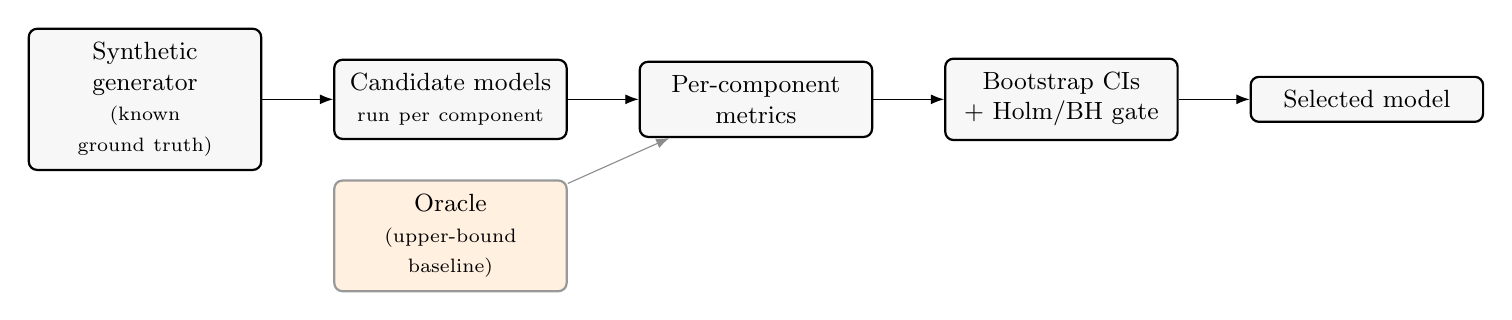
\begin{tikzpicture}[node distance=5mm and 9mm, font=\small, >=Latex,
  b/.style={draw, rounded corners=3pt, line width=0.8pt, align=center, inner sep=5pt, text width=2.6cm, fill=black!3}]
\node[b] (G) {Synthetic generator\\\scriptsize (known ground truth)};
\node[b, right=of G] (M) {Candidate models\\\scriptsize run per component};
\node[b, right=of M] (E) {Per-component metrics};
\node[b, right=of E] (S) {Bootstrap CIs\\$+$ Holm/BH gate};
\node[b, right=of S] (W) {Selected model};
\draw[->] (G) -- (M); \draw[->] (M) -- (E); \draw[->] (E) -- (S); \draw[->] (S) -- (W);
\node[b, below=of M, fill=orange!12, draw=black!40] (O) {Oracle\\\scriptsize (upper-bound baseline)};
\draw[->, draw=black!45] (O) -- (E);
\end{tikzpicture}%
}
\caption{The offline comparison pipeline. The synthetic generator supplies ground truth; each candidate is scored on per-component metrics; a bootstrap confidence interval and Holm/Benjamini--Hochberg correction gate the result before a model is selected. The oracle is an upper-bound reference, not a deployable method.}
\label{fig:pipeline}
\end{figure}

Each component is scored on metrics appropriate to it, defined in Table~\ref{tab:metrics}. Every reported comparison carries a bootstrap confidence interval on the difference between a candidate and the incumbent, and a Holm or Benjamini--Hochberg correction is applied across the family of comparisons so that a win survives multiple-comparison scrutiny. An oracle baseline, which is given the planted ground truth, is included as an upper bound on achievable performance; it is a reference ceiling and is never treated as a deployable method.

\begin{table}[htbp]
\centering
\footnotesize
\caption{Evaluation metrics by component.}
\label{tab:metrics}
\begin{tabular}{p{3.0cm} p{9.0cm}}
\toprule
\textbf{Component} & \textbf{Metrics} \\
\midrule
Pace calibration & Mean absolute error of the recovered pace against the planted pace \\
Change detection & Detection latency after a planted shift, and the false-alarm rate \\
Progress projection & Coverage of the 95\% interval against nominal, and point error in days \\
Schedule generation & Deadline drift and the number of capacity violations \\
\bottomrule
\end{tabular}
\end{table}

\section{System Design and Evolution}
The system did not arrive at its current shape in one step, and the path is worth recording because it explains why the delivered scheduler differs from the one the comparison favoured.

The starting point was the predict-then-optimize architecture of the base paper~\cite{islam2024}, in which a predictive model estimates the learner's pace and an optimizer turns the estimate into a schedule. The initial design realised this literally. The intelligence service ran calibration, detection, projection, and a constraint-based schedule generator, and the generator packed each material onto a specific calendar day, producing the dated slot grid shown in Figure~\ref{fig:arch-initial}. A replan re-ran the packer on the service and returned a new grid.

\begin{figure}[htbp]
\centering
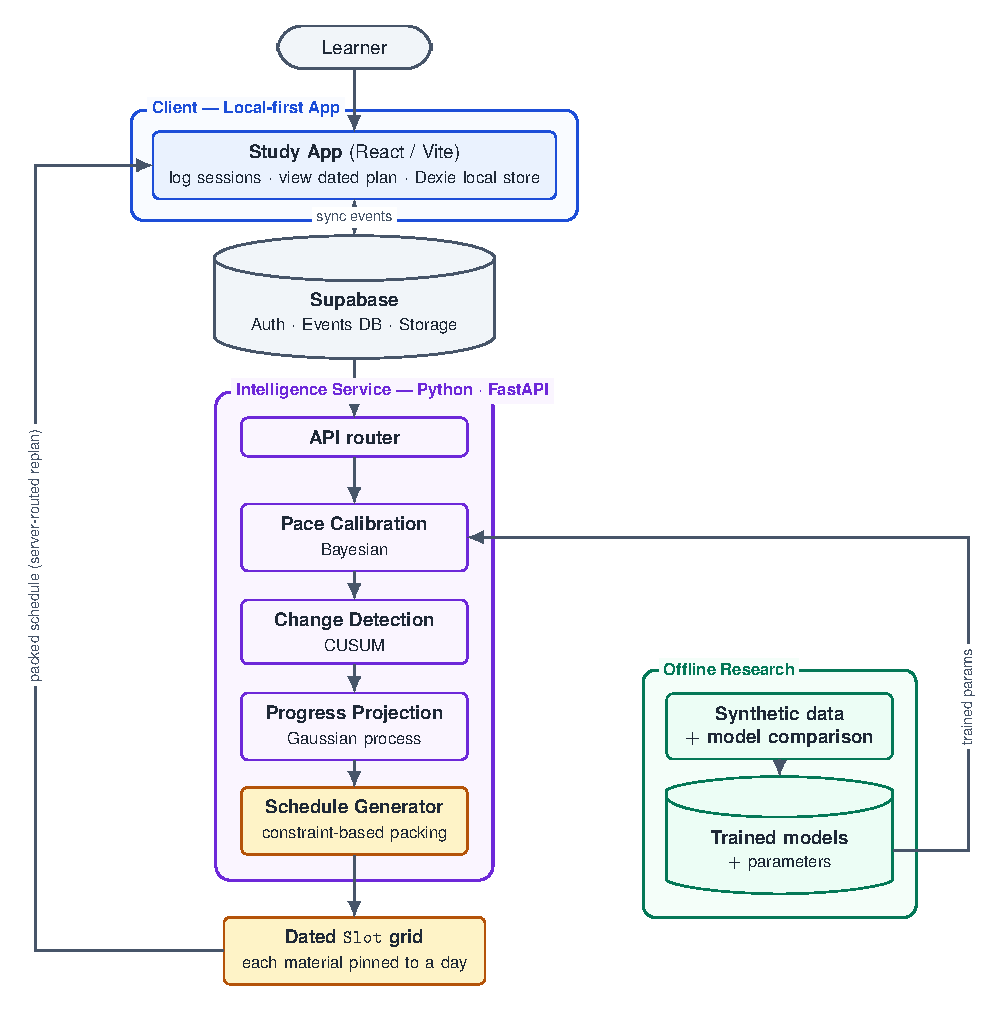
\includegraphics[width=0.66\textwidth]{arch_initial.pdf}
\caption{Initial design (predict-then-optimize). The intelligence service runs all four components, and the schedule generator packs each material onto a fixed day, returning a dated \texttt{Slot} grid; a replan re-runs the packer on the service.}
\label{fig:arch-initial}
\end{figure}

This design proved brittle in use. Pinning materials to fixed days created boundary and tie cases at the edges of the packing that were awkward to resolve, and the rigid day-by-day grid worked against the central goal of continuous replanning: every change to the learner's pace forced a re-pack of the whole grid. The problem the packer solved, deciding exactly which material to study on which day, was also not the problem the learner actually had, which was knowing whether they were on track and what to do next.

The design was therefore revised. The scheduling question was re-examined on a revised synthetic regime that models the new interaction pattern, and the calibration, detection, and projection models were confirmed to transfer to it. The prescriptive packer was retired in favour of a capacity-based booking model: the plan holds blank bookings, each carrying a date and a duration, and the learner picks a material at the start of a session. The engine's job shrinks from packing a grid to estimating a capacity and projecting a finish date. Figure~\ref{fig:arch-revised} shows the resulting architecture.

\begin{figure}[htbp]
\centering
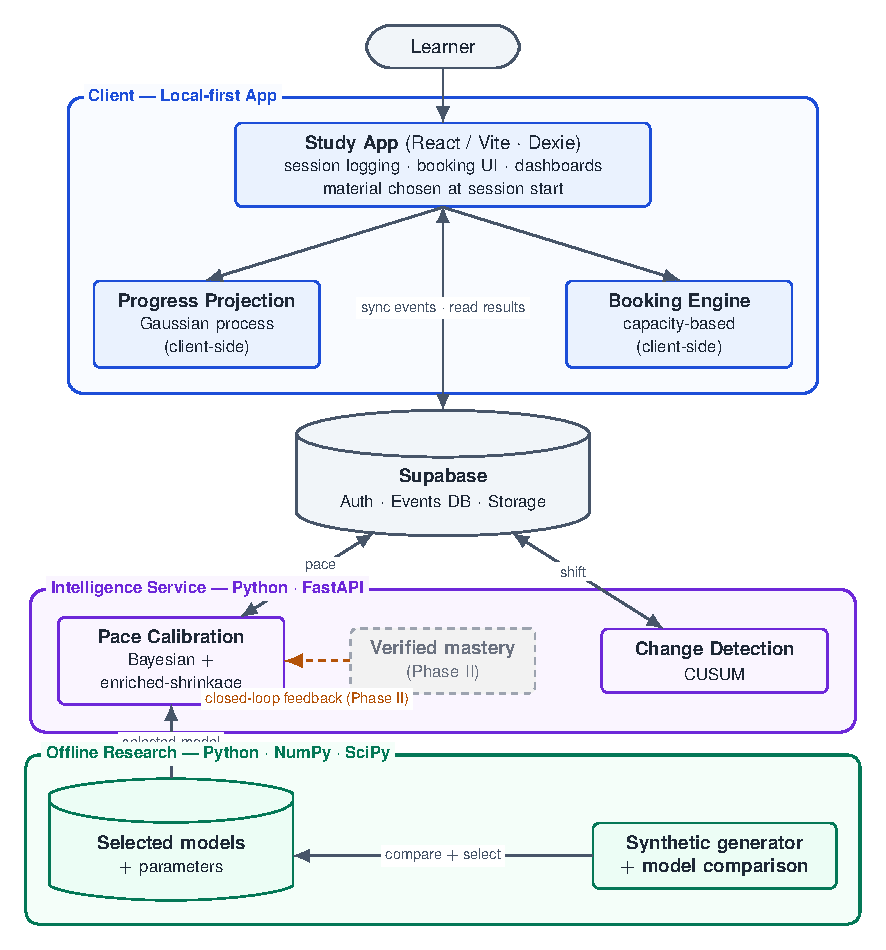
\includegraphics[width=0.74\textwidth]{arch_revised.pdf}
\caption{Revised design (capacity-based booking), the delivered system. Progress projection and the booking engine run client-side; Bayesian and enriched-shrinkage calibration and CUSUM detection run in the Python service; Supabase is the data hub; the offline research pipeline supplies the selected models. The closed-loop feedback from verified mastery is drawn dashed as Phase-II work.}
\label{fig:arch-revised}
\end{figure}

\section{System Architecture}
The delivered system is organised into three tiers, shown in Figure~\ref{fig:arch-revised}, with computation deliberately split between the client and the service according to what each part needs.

The client is a local-first single-page application built with React and Vite, storing every event in a per-user IndexedDB database through Dexie. It owns the parts of the system that derive directly from the learner's local event log: session logging, the booking user interface, the dashboards, the Gaussian-process progress projection, and the capacity-based booking engine. Running these client-side keeps the core loop responsive and available offline. The intelligence service is a Python and FastAPI application that hosts the parts that fit a statistical model to accumulated data: Bayesian and enriched-shrinkage pace calibration and CUSUM change detection. The client calls the service over HTTP, and every request carries a signed token that the service verifies before any model runs. The division follows a simple rule: computation that fits a model to history runs on the service, and computation that derives a view from the local event log runs on the client. Supabase sits between the two as the data hub, providing authentication, the event database, and object storage, with each learner's data isolated by row-level security. An offline research pipeline, described in Section~4.3, supplies the trained models and parameters that the calibrator uses. The closed-loop feedback from verified mastery back into calibration, shown dashed in Figure~\ref{fig:arch-revised}, is the principal Phase-II extension and is not part of the delivered Phase-I system.

\chapter{Implementation Details}
This chapter describes how the system was built. Section~5.1 states the development environment. Section~5.2 describes the datasets and their sources. Section~5.3 describes the model implementation and how the client and service share it. Section~5.4 records the evaluation metrics and the steps taken for reproducibility. Section~5.5 presents the delivered application.

\section{Development Environment}
The project is a single repository with two overlapping workspaces. A pnpm workspace holds the TypeScript client and the shared client-side engines, and a uv workspace holds the Python packages, the intelligence service, and the offline research code. The two coexist so that the research code can import the same Python engines the service runs, which keeps the evaluated code and the shipped code identical. Table~\ref{tab:tools} lists the environment.

\begin{table}[htbp]
\centering
\footnotesize
\caption{Development environment: tools and libraries.}
\label{tab:tools}
\begin{tabular}{p{4.0cm} p{8.4cm}}
\toprule
\textbf{Concern} & \textbf{Technology} \\
\midrule
Client language and build & TypeScript, Vite, pnpm workspace \\
Client UI & React~19 \\
Local-first storage & Dexie over IndexedDB \\
Intelligence service & Python~3.12, FastAPI, Uvicorn \\
Scientific stack & NumPy, SciPy \\
Service authentication & PyJWT, verifying Supabase-issued tokens \\
Containerisation & Docker via Colima \\
Python workspace & uv \\
JavaScript testing & Vitest, fast-check (property tests), Playwright (end-to-end) \\
Python testing and linting & pytest, ruff \\
Backend and hosting & Supabase (auth, database, storage), Vercel \\
\bottomrule
\end{tabular}
\end{table}

\section{Datasets and Their Sources}
Because a single learner's real log cannot supply a known ground truth, the comparison in Chapter~6 is run on synthetic data whose properties are planted and therefore known. Table~\ref{tab:datasets} lists the datasets and the role each plays.

The synthetic generator produces study histories in which the learner's true pace, the timing and size of any regime shift, and the completion behaviour are set explicitly. So that the synthetic regime resembles real behaviour rather than an arbitrary one, its parameters were calibrated against the Open University Learning Analytics Dataset (OULAD), a large public dataset of learner activity. The OULAD is used only to calibrate the generator's realism; it is not used as a direct benchmark. A revised generator regime models the booking interaction pattern introduced by the redesign of Section~4.4, and the selected models were re-checked against it. Real single-learner logs are reserved for the longitudinal validation planned in Phase~II and are not used in Phase~I.

\begin{table}[htbp]
\centering
\footnotesize
\caption{Datasets used in Phase~I and their sources.}
\label{tab:datasets}
\begin{tabular}{p{3.6cm} p{3.8cm} p{5.0cm}}
\toprule
\textbf{Dataset} & \textbf{Source} & \textbf{Role} \\
\midrule
Synthetic study histories & Generated in-repository & Primary ground truth for the component comparison; plants pace, shifts, and learner archetypes \\
OULAD & Public (Open University) & Calibrates the synthetic generator's realism regime; not a direct benchmark \\
Revised (decoupled) regime & Generated in-repository & Re-validates the selected models under the booking interaction model \\
Real single-learner log & The candidate's own sessions & Phase-II longitudinal validation; not used in Phase~I \\
\bottomrule
\end{tabular}
\end{table}

\section{Model Implementation}
The algorithms are implemented once in behaviour and twice in code. The client-side engines are written in TypeScript, and a Python mirror of each engine is exposed through the intelligence service. The two implementations are kept aligned by a golden-fixture parity harness: the TypeScript engines emit reference inputs and outputs, and a Python test replays each input and asserts numeric equality to a tight tolerance. The shared numeric constants, such as the Bayesian prior, the CUSUM slack and threshold factors, and the Gaussian-process length scale, are held identical on both sides.

The split between client and service follows the architecture of Figure~\ref{fig:arch-revised}. Computation that fits a statistical model to accumulated history runs on the service: Bayesian and enriched-shrinkage pace calibration and CUSUM change detection, reached over HTTP at a calibration endpoint that verifies a signed token before running. Computation that derives a view from the local event log runs in the browser: the Gaussian-process projection, the burn-up and streak summaries, and the capacity-based booking engine. The offline research harness imports the production Python engines as candidates rather than re-implementing them, so a result measured offline is a result about the shipped code. Listing~\ref{lst:cusum} shows the shipped change detector, which realises Equation~\eqref{eq:cusum}, and Table~\ref{tab:packages} lists the main packages.

\noindent\begin{minipage}{\linewidth}
\begin{lstlisting}[language=Python, caption={The shipped one-sided CUSUM detector, realising Equation~\eqref{eq:cusum}.}, label={lst:cusum}]
def run_cusum(series, mu0, k, h):
    """Return the index of the first alarm, or None if no shift is detected."""
    s = 0.0
    for t, x in enumerate(series):
        s = max(0.0, s + (x - mu0) - k)   # accumulate deviation, floored at zero
        if s > h:                          # threshold crossed -> shift detected
            return t
    return None
\end{lstlisting}
\end{minipage}

\begin{table}[H]
\centering
\footnotesize
\caption{Main packages and their roles.}
\label{tab:packages}
\begin{tabular}{p{4.8cm} p{7.6cm}}
\toprule
\textbf{Package / module} & \textbf{Role} \\
\midrule
\texttt{packages/progress} (TS) & Client engine: Gaussian-process projection, burn-up, streak, calibration mirror \\
\texttt{packages/roadmap-engine} (TS) & Client booking and roadmap generation \\
\texttt{packages/py-progress} (Py) & Python mirror: Bayesian and enriched-shrinkage calibration, CUSUM, Gaussian process \\
\texttt{packages/py-roadmap-engine} (Py) & Python mirror of the roadmap engine \\
\texttt{services/intelligence} (Py) & FastAPI service exposing calibration over HTTP, token-verified \\
\texttt{research/comparison} (Py) & Offline harness importing the production engines as candidates \\
\bottomrule
\end{tabular}
\end{table}

\section{Evaluation Metrics and Reproducibility}
The metrics used to score each component are defined in Table~\ref{tab:metrics} of Chapter~4: recovery error for calibration, detection latency and false-alarm rate for change detection, interval coverage and point error for projection, and deadline drift and capacity violations for scheduling. This section records how they are computed and how the results are made reproducible.

Every reported comparison is accompanied by a bootstrap confidence interval on the difference between a candidate and the incumbent, estimated by resampling learners with replacement. Across the family of comparisons a Holm or Benjamini--Hochberg correction is applied, so that a claimed win survives multiple-comparison scrutiny rather than arising from testing many candidates. A result is reported only when it passes a set of credibility checks that guard against degenerate or unstable cells. The pipeline is driven by fixed random seeds and a small set of make targets, so that the dataset, the comparison, and the figures regenerate deterministically, and each generated figure and table carries a provenance stamp recording the run that produced it.

\section{The Phase-1 Application}
The selected models are not left as an offline result. They are realised in a working, local-first web application for a single self-directed learner, which this section presents in full. The application is organised around four capabilities, and the section follows them. Section~5.5.1 covers plan creation, where onboarding turns a deadline, a weekly capacity, and a set of materials into a booked schedule. Section~5.5.2 covers study execution, the session runtime under which the work is done and recorded. Section~5.5.3 covers progress and adaptation, the dashboards that report calibrated pace and projected completion and the screen that adjusts the plan. Section~5.5.4 covers plan lifecycle, the calendar and dashboard that track a plan from draft to completion. Section~5.5.5 describes the local-first data architecture underneath all four. Every screenshot in this section is captured from the running application.

\subsection{Plan Creation: Onboarding and Roadmap Generation}
A new learner is taken through a four-step onboarding wizard that collects the planner's inputs and produces an initial schedule. The first step records the target deadline and an optional statement of purpose. The second records a weekly study capacity, divided by default in a 60/40 ratio between weekdays and weekends over a chosen set of study days. The third collects the study materials: a material is added by pasting a link, which a lightweight classifier resolves into a YouTube video, a playlist, an article, or a manual entry, and each material is assigned a role of anchor, foundation, or practice that later governs its ordering. The fourth step presents a read-only summary before the plan is committed. Figure~\ref{fig:app-onboarding} shows the generated plan at the close of onboarding.

From these inputs the client-side roadmap engine generates the schedule. Rather than packing each day with a prescribed material, as the retired constraint-based design did (Section~4.4), the engine lays capacity-sized bookings across the study days between the start date and the deadline, and leaves the specific material to be chosen at the start of each session. The wizard writes its state to the local event log on every step, so a learner who closes the tab midway resumes where they stopped instead of starting over. Committing the plan emits the events the rest of the system reads: a \texttt{MaterialAdded} event for each material, a \texttt{RoadmapCreated} event for the plan, a \texttt{SessionBooked} event for each booking, and an \texttt{OnboardingCompleted} event that admits the learner to the main application.

\begin{figure}[htbp]
\centering
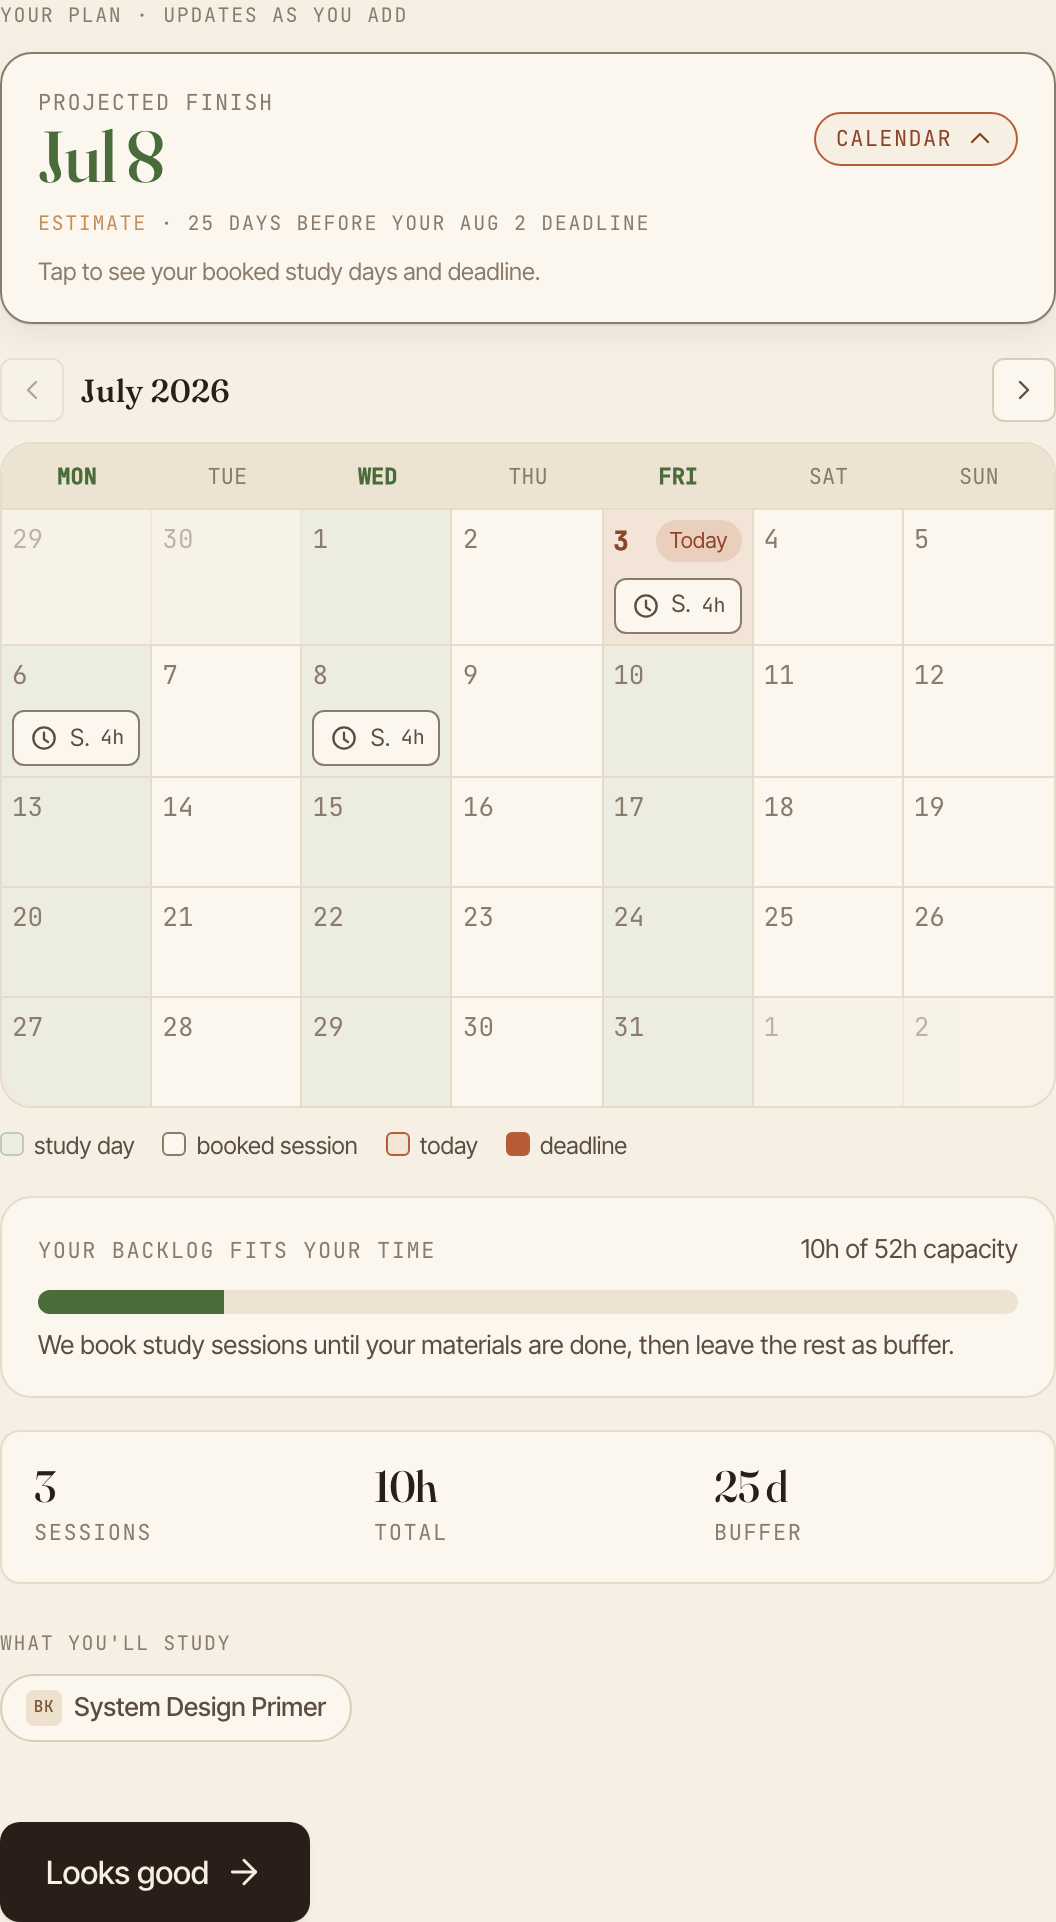
\includegraphics[width=0.85\linewidth, height=0.42\textheight, keepaspectratio]{screenshots/app_onboarding_plan.png}
\caption{Onboarding: the generated booking plan produced from the learner's deadline, weekly capacity, and materials.}
\label{fig:app-onboarding}
\end{figure}

\subsection{Study Execution: the Session Runtime}
When it is time to study, the learner starts a session from the plan and chooses the material to work on at that moment. The session runs under a timer with optional Pomodoro intervals of fifty working minutes separated by ten-minute breaks. The interval clock advances on wall-clock time, so a break that is due still arrives even after the timer has been paused. A YouTube material plays in an embedded player whose position is tracked, so that a multi-video playlist resumes at the point it reached, while an article opens in a separate tab and is timed alongside. Figure~\ref{fig:app-session} shows a session in progress.

The runtime is governed by a small state machine over idle, active, and paused states that also recognises a stale session, such as a timer left running overnight or a tab hidden for several minutes, and offers a recovery path rather than recording a spurious multi-hour session. When a session ends it records the minutes actually worked, the number of pauses, the Pomodoro blocks completed, and the position reached in each material, and this record is what later feeds the pace calibration and the progress views. A session can also be flagged as exceptional, marking an atypical day so that it does not distort the pace estimate.

\begin{figure}[htbp]
\centering
\includegraphics[width=0.85\linewidth, height=0.42\textheight, keepaspectratio]{screenshots/app_session.png}
\caption{A study session in progress, with the timer and material chosen at the start of the session.}
\label{fig:app-session}
\end{figure}

\subsection{Progress and Adaptation: Home, Week, and Replan}
Between sessions the learner sees how the plan is tracking. The Home dashboard (Figure~\ref{fig:app-home}) summarises the current state in a single view: the next booking to act on, the current and best study streak, the calibrated pace, and the projected finish date. The calibrated pace is produced by the intelligence service. The browser sends the session history to a token-verified calibration endpoint, and the Python engine returns the hierarchical-Bayesian estimate refined by the context-aware shrinkage calibrator of Equation~\eqref{eq:enriched}, together with per-role multipliers. The projection and the streak, by contrast, are computed in the browser from the local event log.

\begin{figure}[htbp]
\centering
\includegraphics[width=0.85\linewidth, height=0.42\textheight, keepaspectratio]{screenshots/app_home.png}
\caption{The Home dashboard: up-next booking, streak, calibrated pace, and projected finish date.}
\label{fig:app-home}
\end{figure}

The Week view (Figure~\ref{fig:app-week}) reports a single verdict for the week, ahead, on track, or behind, above a daily-minutes chart and a burn-up projection. The burn-up plots the cumulative minutes actually logged against the planned ramp and overlays the Gaussian-process mean with its 95\% band, falling back to an analytic estimate while fewer than five sessions have accumulated so that the early projection stays stable (Section~4.2). The point at which the band crosses the target line is the projected completion, read against the deadline.

\begin{figure}[htbp]
\centering
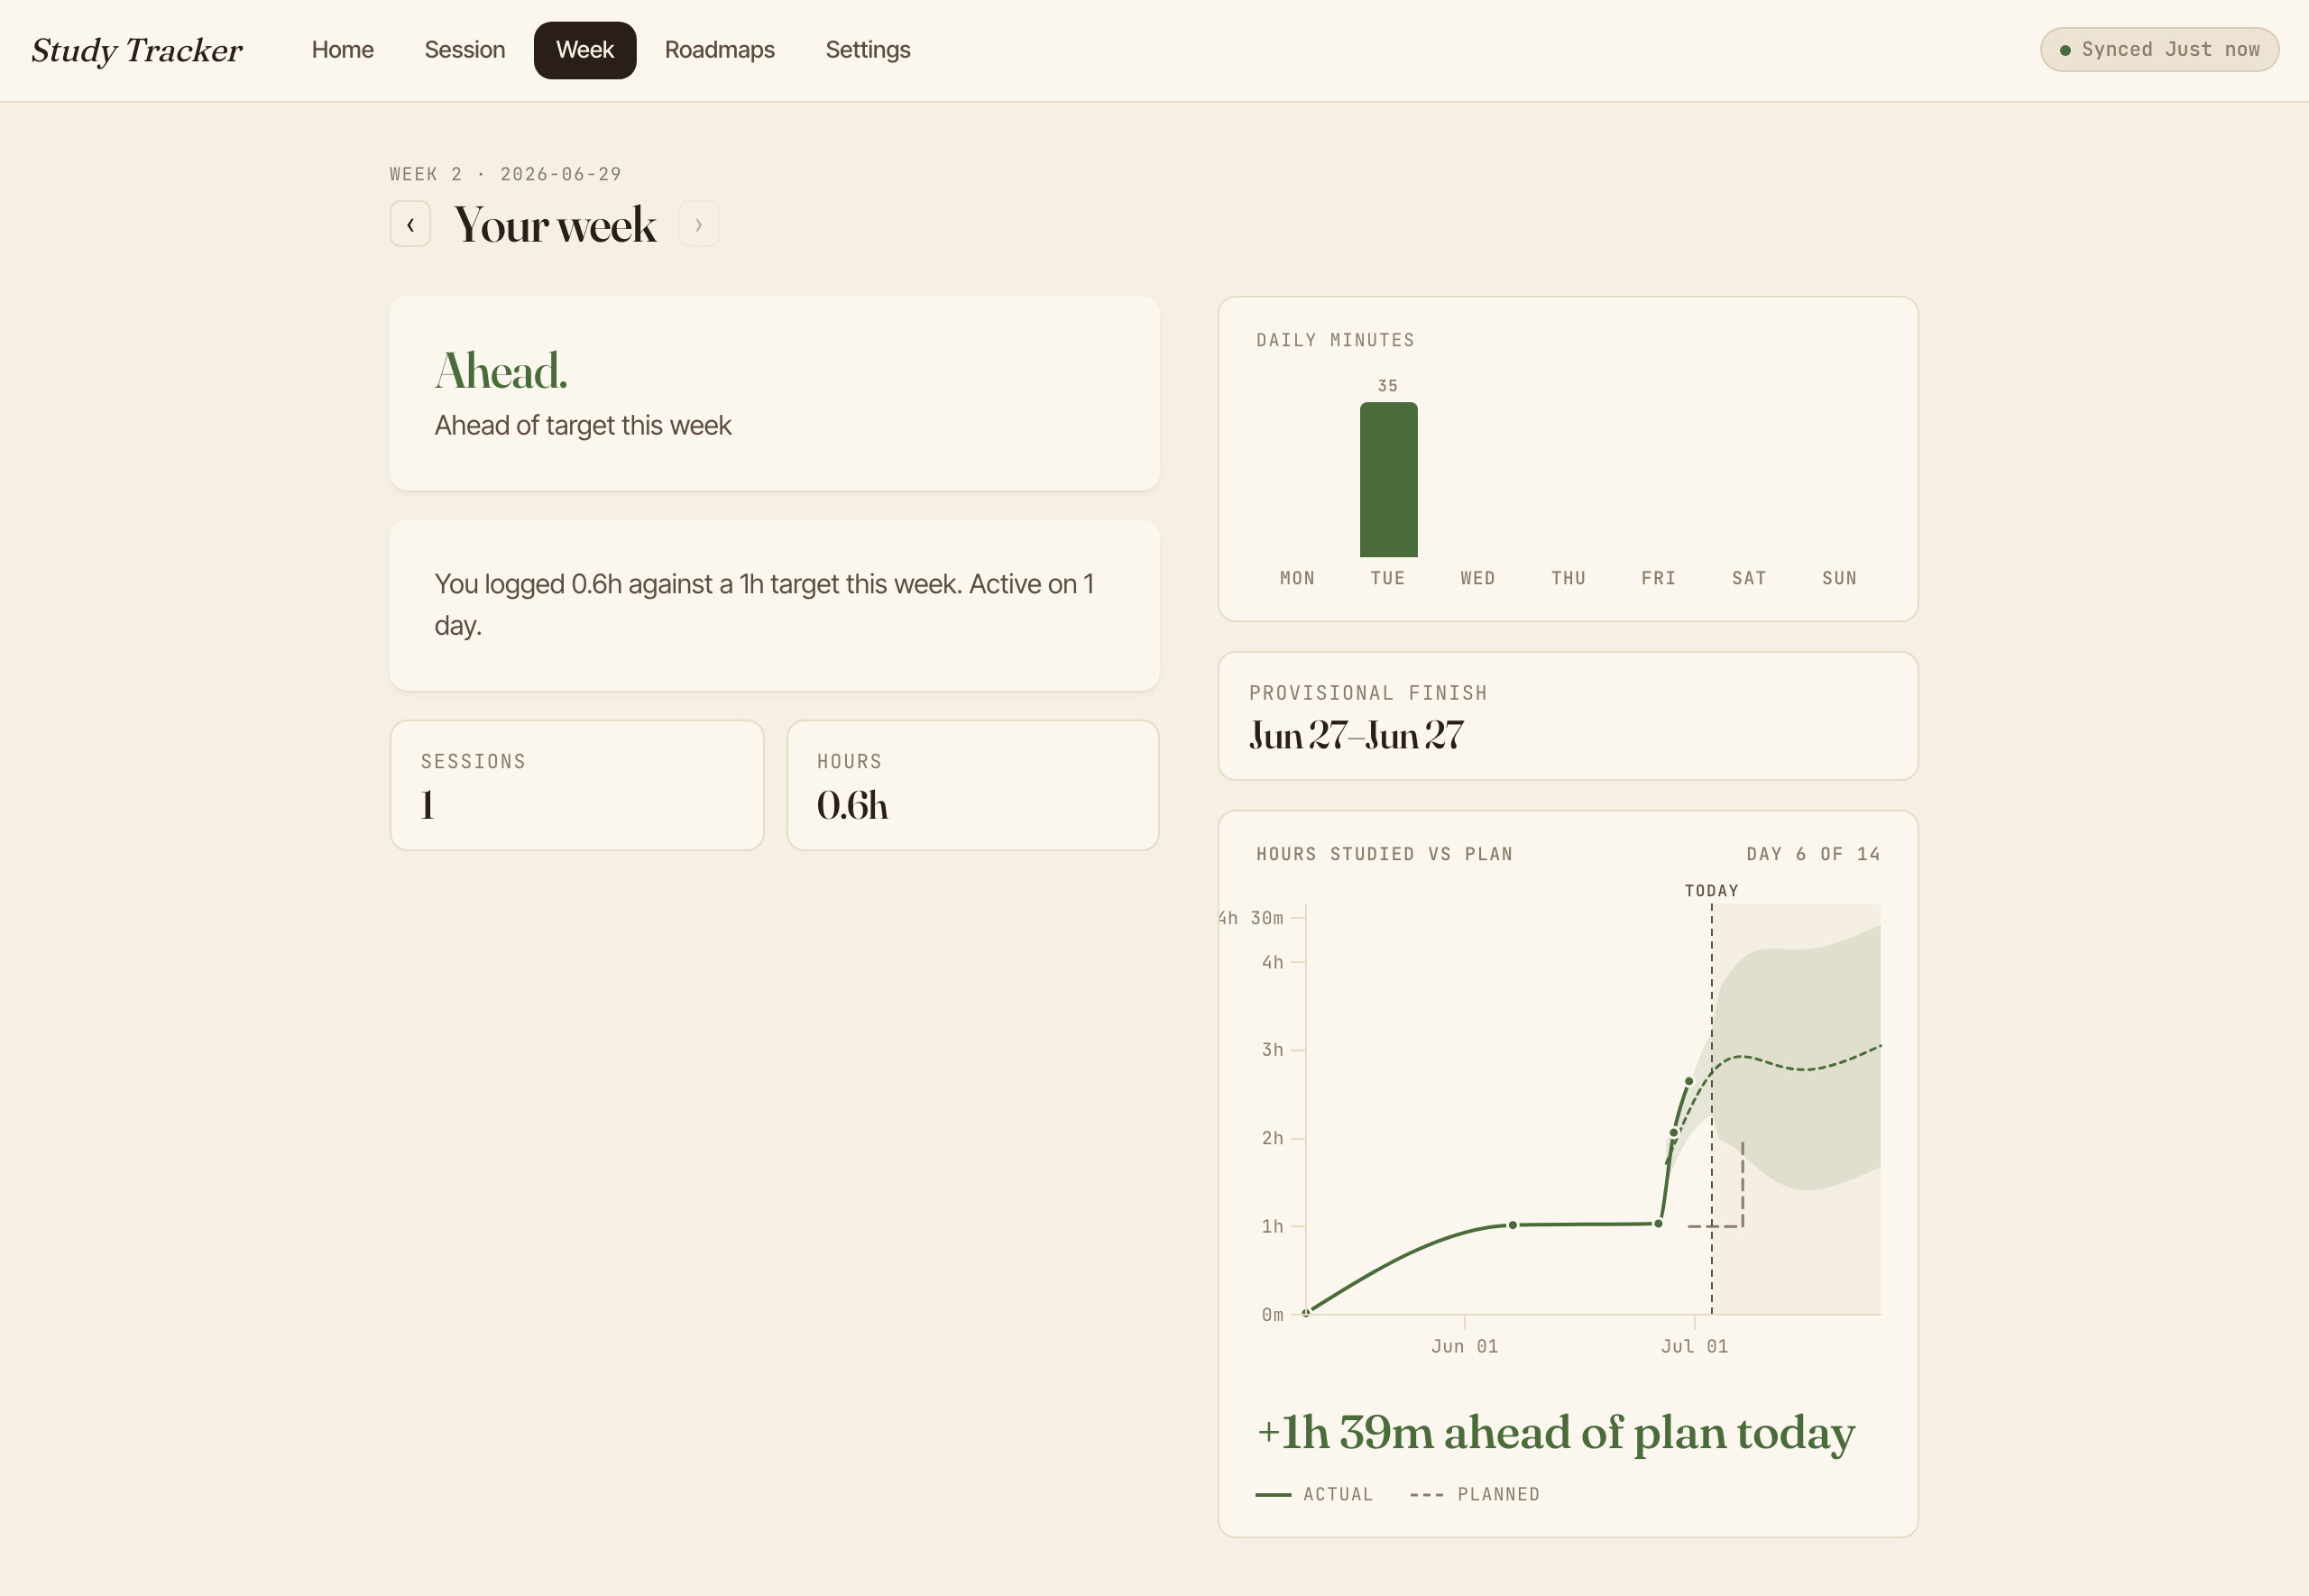
\includegraphics[width=0.85\linewidth, height=0.42\textheight, keepaspectratio]{screenshots/app_week.png}
\caption{The Week view: the week's verdict, the daily-minutes chart, and the burn-up projection.}
\label{fig:app-week}
\end{figure}

When realised pace diverges from the plan, the system does not silently rewrite the schedule. Change detection runs server-side on the same calibration call, and a divergence surfaces as a recalibration prompt that the learner can accept, acknowledge, or defer; the plan is changed only on the learner's instruction, which keeps the loop open (Section~4.1). The Replan screen (Figure~\ref{fig:app-replan}) offers three independent levers for that change: extend or shorten the deadline, raise or lower the weekly hours, or drop and trim materials. Each lever shows its effect on the projected finish date as it is moved, so the trade is visible before it is committed. Confirming a replan re-lays the bookings and records a \texttt{RoadmapReplanned} event that preserves the plan's identity, so its history remains intact.

\begin{figure}[htbp]
\centering
\includegraphics[width=0.85\linewidth, height=0.42\textheight, keepaspectratio]{screenshots/app_replan.png}
\caption{The Replan screen: three levers to adjust the plan when the projection diverges from the deadline.}
\label{fig:app-replan}
\end{figure}

\subsection{Plan Lifecycle: the Roadmap Calendar and Roadmaps Dashboard}
A plan is more than its current week. The Roadmap calendar (Figure~\ref{fig:app-roadmap}) shows the whole plan as a month grid, with study days tinted and each booking placed on its day and coloured by material role. Selecting a day opens a sheet in which the learner can add, edit, or clear a booking and mark how far through a material they have reached. A booking's status, whether unstarted, in progress, completed, trimmed, or interrupted, is derived from the logged sessions rather than stored, so it stays consistent with what actually happened.

\begin{figure}[htbp]
\centering
\includegraphics[width=0.85\linewidth, height=0.42\textheight, keepaspectratio]{screenshots/app_roadmap.png}
\caption{The Roadmap calendar: the plan shown as a month grid of bookings.}
\label{fig:app-roadmap}
\end{figure}

The Roadmaps dashboard (Figure~\ref{fig:app-roadmaps}) tracks plans across their lifecycle. The active plan is shown with its date range and progress, an unfinished onboarding draft is offered for resumption, and completed or abandoned plans are kept in a history that can be reopened read-only. Because a replan preserves the plan's identity, a plan and its successive replans collapse into a single entry rather than appearing as several unrelated plans.

\begin{figure}[htbp]
\centering
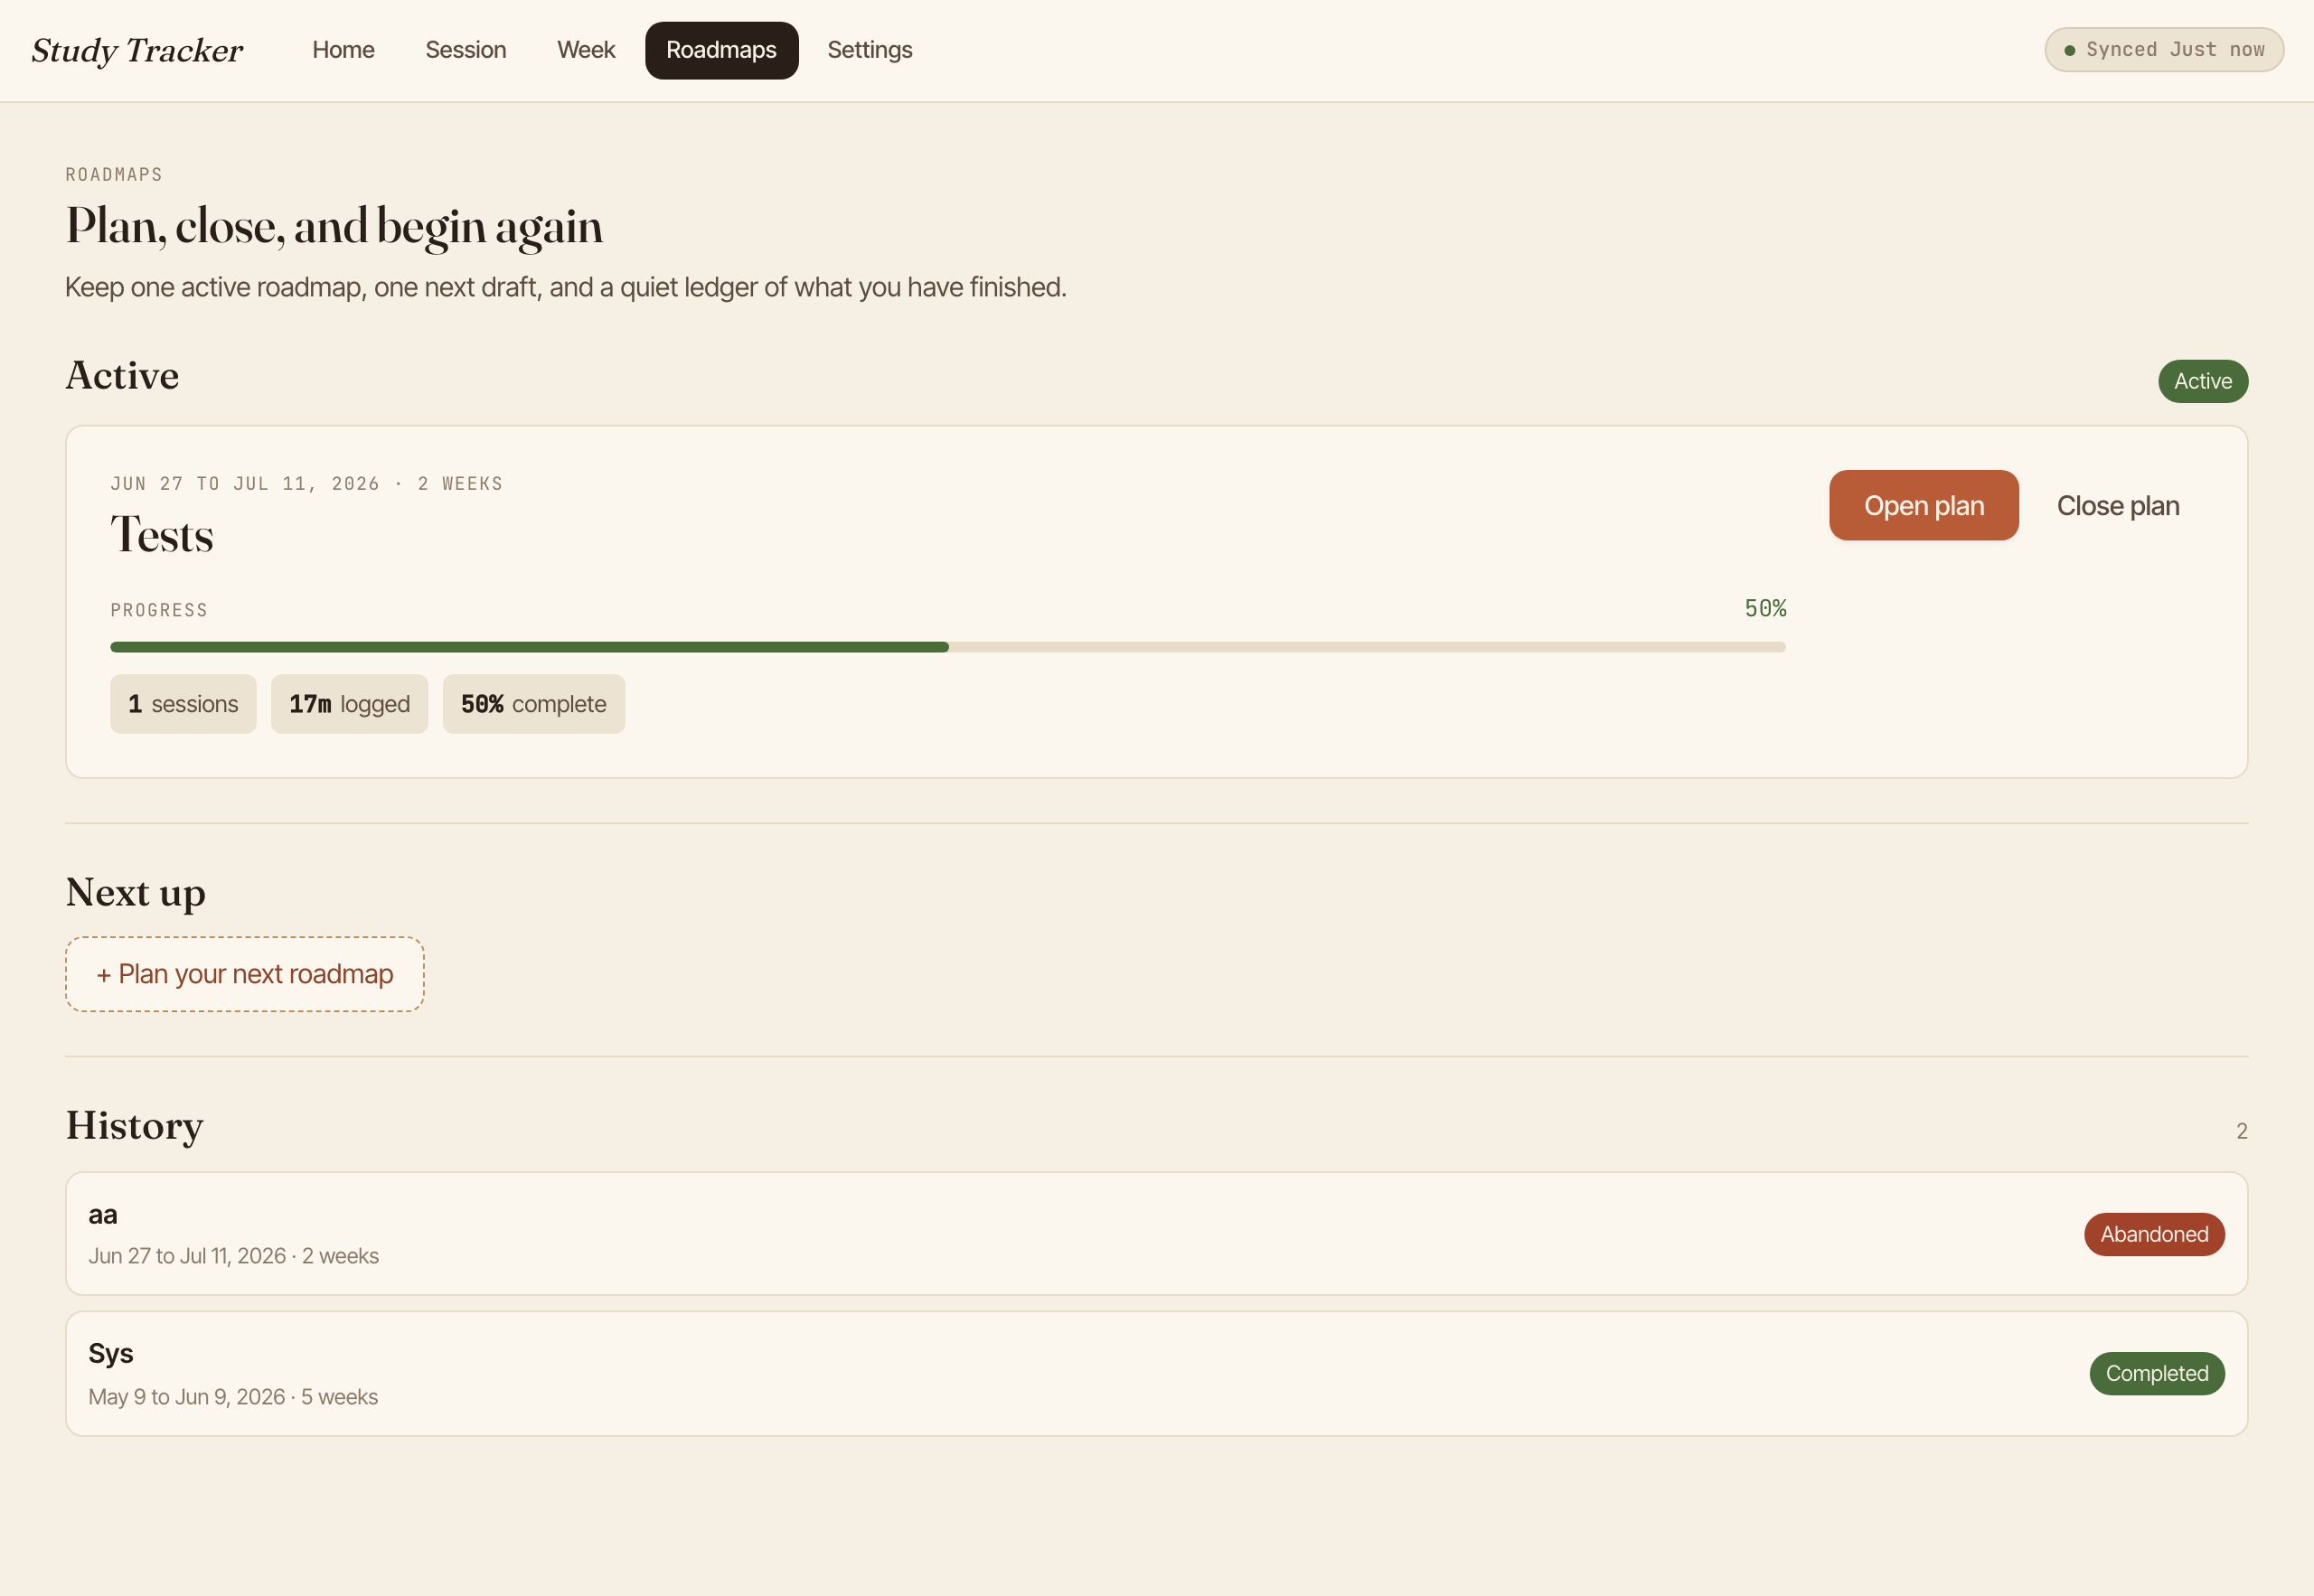
\includegraphics[width=0.85\linewidth, height=0.42\textheight, keepaspectratio]{screenshots/app_roadmaps.png}
\caption{The Roadmaps dashboard: the active plan, drafts, and history over their lifecycle.}
\label{fig:app-roadmaps}
\end{figure}

\subsection{The Local-First Data Architecture}
The four capabilities above rest on a local-first, event-sourced data layer. Every action the learner takes is recorded as an immutable event in a log held in the browser's IndexedDB, and every view, whether a dashboard, the calendar, or a projection, is derived by replaying that log rather than by reading mutable records. Because the log is local, the core loop stays usable without a network connection: reads and writes complete against the local store and reconcile with the cloud when a connection returns. Each signed-in learner has a separate local database keyed by their identity, so two accounts sharing a browser never see each other's data and neither loses its history on sign-out.

Durability to the cloud is provided by a write-ahead queue. Events are enqueued locally and flushed to a Supabase table, and a periodic snapshot of the log is uploaded to object storage, so that a new device restores the full history from the snapshot and then replays only the events recorded since it. In Phase~1 the plan's own events, its creation, its bookings, and any replan, synchronise to the cloud through this queue, while extending the same durability to the stream of events emitted during a live study session is a hardening task carried into Phase~II. The division of computation between this client and the intelligence service follows the architecture of Section~4.5 and Figure~\ref{fig:arch-revised}: model fitting over accumulated history runs in the service, and every view derived from the local log runs in the browser.

\chapter{Results and Discussion}
This chapter reports the offline comparison for each Pillar-A component and discusses what the numbers mean for the delivered system. All results are computed on the synthetic ground-truth data described in Section~5.2, over 200 seeds and held-out learner archetypes, with bootstrap confidence intervals and Holm/Benjamini--Hochberg correction as described in Section~4.3. Each component is reported for both the initial (frozen) synthetic regime and the revised (decoupled) regime that matches the booking model, so that the transfer of a result across the redesign is visible. Throughout, the oracle is the upper-bound reference that is given the planted ground truth; it is never a deployable method. Section~6.1 covers pace calibration, Section~6.2 change detection, Section~6.3 progress projection, Section~6.4 schedule generation, and Section~6.5 discusses the results together.

\section{Pace Calibration}
Table~\ref{tab:res-cal} reports the mean recovery error of the pace estimate against the planted pace, by history-length band. The reading is deliberately honest: on this retrospective metric the structured Bayesian variants do not separate from the hierarchical-Bayesian incumbent, and the incumbent is in fact the strongest deployable method at the longest histories. The context-aware enriched-shrinkage calibrator improves on the incumbent on short histories, where its shrinkage toward a population prior helps most, but it is worse at the maximum band. This is an honest null for the structured calibrators on recovery error.

\begin{table}[htbp]
\centering
\footnotesize
\caption{Pace calibration: mean recovery error (lower is better) by history-length band, frozen regime. The oracle is the upper-bound reference.}
\label{tab:res-cal}
\begin{tabular}{l r r r}
\toprule
\textbf{Method} & \textbf{Short} & \textbf{Medium} & \textbf{Long} \\
\midrule
Oracle (reference ceiling) & 0.000 & 0.000 & 0.000 \\
Enriched-shrinkage (selected) & 0.049 & 0.049 & 0.056 \\
Hierarchical Bayesian (incumbent) & 0.079 & 0.046 & 0.026 \\
Moving average & 0.094 & 0.100 & 0.090 \\
EWMA & 0.115 & 0.124 & 0.107 \\
\bottomrule
\end{tabular}
\end{table}

The reason the enriched-shrinkage calibrator was nonetheless selected is that recovery error is not the quantity the planner acts on. The planner needs a \emph{prospective} pace estimate for the next session, especially when the learner has logged little history. On that prospective metric the enriched-shrinkage calibrator is a robust improvement over the incumbent across every band and both regimes, and the improvement survives Holm correction (Table~\ref{tab:res-cal-ctx}). It is to be noted that this is exactly the low-data regime in which a new learner's plan first needs to adapt, which is why the prospective advantage was judged to matter more than the retrospective null.

\begin{table}[htbp]
\centering
\footnotesize
\caption{Enriched-shrinkage minus hierarchical-Bayesian on the prospective context-prediction error (negative favours enriched-shrinkage), with 95\% bootstrap intervals.}
\label{tab:res-cal-ctx}
\begin{tabular}{l l l}
\toprule
\textbf{Band} & \textbf{Frozen $\Delta$ [95\% CI]} & \textbf{Decoupled $\Delta$ [95\% CI]} \\
\midrule
Short & $-0.0148$ [$-0.0168$, $-0.0127$] & $-0.0145$ [$-0.0155$, $-0.0136$] \\
Medium & $-0.0262$ [$-0.0282$, $-0.0243$] & $-0.0268$ [$-0.0277$, $-0.0258$] \\
Long & $-0.0300$ [$-0.0316$, $-0.0285$] & $-0.0307$ [$-0.0316$, $-0.0299$] \\
\bottomrule
\end{tabular}
\end{table}

\section{Change Detection}
Table~\ref{tab:res-det} reports detection latency and false-alarm rate by shift type on the frozen regime. The comparison is a robust null in the sense that no exotic detector improves on the established CUSUM and critical-slowing-down frontier. CUSUM detects fastest, at roughly one and a half sessions after a shift, at the cost of the highest false-alarm rate; the critical-slowing-down and Page-Hinkley detectors trade latency for far fewer false alarms; the exponentially weighted control chart and the Bayesian online change-point detector are markedly slower; and the ADWIN detector fails to fire at all on this data. Under the combined score that penalises both late detection and false alarms, CUSUM wins on drift shifts in both regimes and is competitive on step shifts, where Page-Hinkley edges it in the frozen regime and CUSUM regains the lead in the decoupled regime.

\begin{table}[htbp]
\centering
\footnotesize
\caption{Change detection: mean detection latency (sessions, lower is better) and false-alarm rate by shift type, frozen regime. ADWIN did not fire on this data.}
\label{tab:res-det}
\begin{tabular}{l r r r r}
\toprule
& \multicolumn{2}{c}{\textbf{Step shift}} & \multicolumn{2}{c}{\textbf{Drift shift}} \\
\cmidrule(lr){2-3}\cmidrule(lr){4-5}
\textbf{Detector} & \textbf{Latency} & \textbf{False-alarm} & \textbf{Latency} & \textbf{False-alarm} \\
\midrule
CUSUM (selected) & 1.43 & 0.312 & 1.36 & 0.296 \\
Critical slowing down & 5.16 & 0.083 & 4.10 & 0.049 \\
Page-Hinkley & 3.03 & 0.149 & 2.39 & 0.139 \\
EWMA control chart & 11.95 & 0.039 & 10.68 & 0.024 \\
Bayesian online change point & 30.59 & 0.009 & 19.43 & 0.011 \\
ADWIN & --- & 0.000 & --- & 0.000 \\
\bottomrule
\end{tabular}
\end{table}

The delivered system ships the single-arm CUSUM. Its higher false-alarm rate is acceptable here because a detected shift raises a recalibration prompt rather than triggering an automatic replan (Section~4.1): a false alarm costs the learner a dismissal, not a wrongly regenerated plan, whereas a late detection costs adaptation time. Fast detection with human confirmation is the better trade for this design.

\section{Progress Projection}
Table~\ref{tab:res-proj} reports the interval coverage and point error of the projection by history-length band, for both regimes. The point error is the same for the plain Gaussian process and the conformal method because the conformal step only rescales the interval width, not the point estimate. The headline result is a coverage failure of the raw Gaussian-process interval: against a nominal 95\%, the plain interval covers only 19\% to 49\% of the time, and the shortfall worsens as the horizon lengthens. The split-conformal correction restores coverage to between 94\% and 99\%, at the same point error. Figure~\ref{fig:res-coverage} shows the gap.

\begin{table}[htbp]
\centering
\footnotesize
\caption{Progress projection: interval coverage (nominal 0.95) and point error in days, by band. Point error is shared between the plain and conformal intervals.}
\label{tab:res-proj}
\begin{tabular}{l r r r r r}
\toprule
& \multicolumn{2}{c}{\textbf{Coverage (frozen)}} & \multicolumn{2}{c}{\textbf{Coverage (decoupled)}} & \textbf{Point error} \\
\cmidrule(lr){2-3}\cmidrule(lr){4-5}
\textbf{Band} & \textbf{Plain GP} & \textbf{Conformal} & \textbf{Plain GP} & \textbf{Conformal} & \textbf{(days, frozen)} \\
\midrule
Short & 0.438 & 0.969 & 0.494 & 0.989 & 2.15 \\
Medium & 0.291 & 0.990 & 0.277 & 0.988 & 9.45 \\
Long & 0.187 & 0.937 & 0.183 & 0.988 & 20.17 \\
\bottomrule
\end{tabular}
\end{table}

\begin{figure}[htbp]
\centering
\resizebox{0.85\linewidth}{!}{%
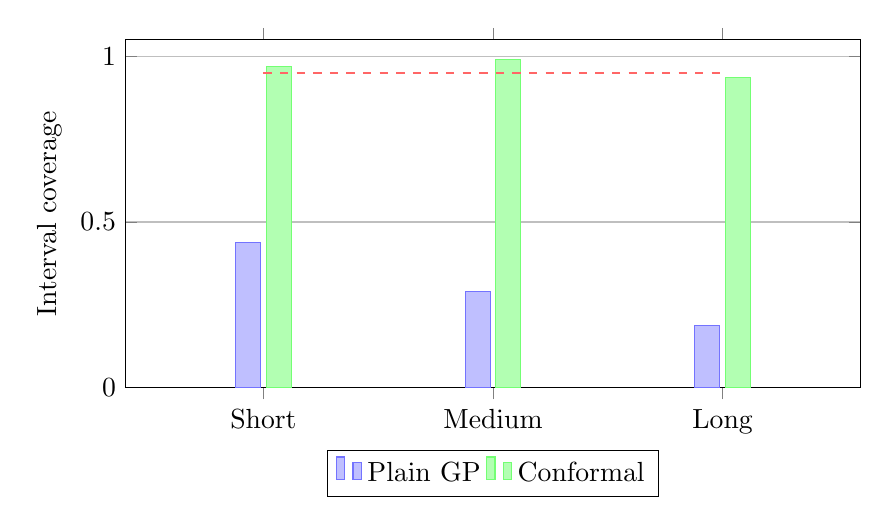
\begin{tikzpicture}
\begin{axis}[ybar, bar width=9pt, width=0.9\linewidth, height=6cm, ymin=0, ymax=1.05,
  ylabel={Interval coverage}, symbolic x coords={Short, Medium, Long}, xtick=data,
  legend style={at={(0.5,-0.18)}, anchor=north, legend columns=-1}, ymajorgrids, enlarge x limits=0.3]
\addplot[fill=blue!25, draw=blue!55] coordinates {(Short,0.438) (Medium,0.291) (Long,0.187)};
\addplot[fill=green!30, draw=green!55] coordinates {(Short,0.969) (Medium,0.990) (Long,0.937)};
\draw[dashed, thick, red!60] (axis cs:Short,0.95) -- (axis cs:Long,0.95);
\legend{Plain GP, Conformal}
\end{axis}
\end{tikzpicture}%
}
\caption{Interval coverage against the nominal 0.95 (dashed) by history-length band, frozen regime. The plain Gaussian-process interval under-covers badly; the split-conformal correction restores near-nominal coverage.}
\label{fig:res-coverage}
\end{figure}

The delivered system ships the Gaussian process with a cold-start composite that falls back to an analytic estimate when the learner has too few sessions for the process to be trusted; on the decoupled regime this composite improves cold-start coverage over the raw Gaussian process, for example lifting short-history coverage from 0.19 to 0.44. The split-conformal correction, which is the fix for the data-rich under-coverage in Table~\ref{tab:res-proj}, is validated here but is recorded as a follow-up not yet shipped; the delivered projection therefore reports an honest but under-covering interval past the cold-start threshold, a limitation returned to in Section~6.5 and Chapter~7.

\section{Schedule Generation}
Table~\ref{tab:res-sch} reports deadline drift and capacity violations by material mix on the reality-matched regime. The dynamic-programming capacity allocator minimises deadline drift in every mix, and the margin over the greedy incumbent grows sharply with the number of interleaved material roles: on the full anchor-plus-foundation-plus-practice mix the greedy incumbent drifts by roughly 39 days while the dynamic-programming allocator drifts by about 8, a difference of $-30.93$ days [$-31.70$, $-30.19$]. All candidates respect the prerequisite ordering and, apart from a negligible rate for the rule-based baseline, incur no capacity violations.

\begin{table}[htbp]
\centering
\footnotesize
\caption{Schedule generation: mean absolute deadline drift (days) by material mix, reality-matched regime. Capacity violations were zero for the selected allocator.}
\label{tab:res-sch}
\begin{tabular}{l r r r}
\toprule
\textbf{Material mix} & \textbf{DP capacity} & \textbf{Greedy incumbent} & \textbf{$\Delta$ drift [95\% CI]} \\
\midrule
Anchor & 1.73 & 3.11 & $-1.21$ [$-1.71$, $-0.72$] \\
Anchor + foundation & 2.35 & 3.65 & $-1.07$ [$-1.58$, $-0.55$] \\
Anchor + practice & 3.91 & 5.94 & $-2.03$ [$-2.71$, $-1.39$] \\
Anchor + foundation + practice & 8.30 & 38.98 & $-30.93$ [$-31.70$, $-30.19$] \\
\bottomrule
\end{tabular}
\end{table}

This is a genuine win for the dynamic-programming allocator, and it is the one component result the delivered system does not act on. As recorded in Section~4.4, the day-by-day packing formulation these schedulers share was retired during development in favour of the capacity-based booking model, because rigid packing was brittle at day boundaries and worked against continuous replanning. The scheduling comparison is therefore reported as an evaluated result that informed a design decision, not as the behaviour of the shipped scheduler.

\section{Discussion}
Read together, the results separate into honest nulls, real wins, and validated refinements not yet shipped. Calibration is a null on retrospective recovery error and a real, Holm-surviving win for the enriched-shrinkage calibrator on the prospective, short-history regime the planner actually depends on. Detection is a robust null: nothing beats the CUSUM frontier, and the shipped CUSUM is the fastest detector, which suits a human-confirmed prompt. Projection produces the clearest finding of the chapter, that the raw Gaussian-process interval under-covers severely and that a split-conformal correction fixes it; the correction is validated but deferred, so interval calibration past the cold-start threshold is a known limitation. Scheduling is a real win for a method the system deliberately does not ship, because the problem it solved was removed by the redesign.

Two cross-cutting points support the credibility of these results. First, the selected models transfer across the two synthetic regimes: the enriched-shrinkage advantage on prospective error and the projection coverage failure both hold from the frozen regime to the decoupled regime that matches the booking model, so the findings are not artefacts of one data-generating process. Second, all of this rests on synthetic data with known ground truth; the synthetic setting is what makes latency, coverage, and recovery measurable at all, but it is not a substitute for real use. Validation on a single learner's own logged sessions is deferred to Phase~II, as set out in Chapter~7.

\chapter{Conclusion and Future Work}
This chapter concludes Phase~I and sets out the work planned for Phase~II. Section~7.1 summarises what was built and found. Section~7.2 describes the Phase-II extensions.

\section{Conclusion}
This report has presented Phase~I of an adaptive study-planning system for self-directed learners. The system estimates a learner's pace with hierarchical Bayesian calibration and a context-aware enriched-shrinkage model, detects behavioural shifts with CUSUM, projects the completion date with a Gaussian process and a cold-start composite, and regenerates the plan with a capacity-based booking model. These components are realised in a working, local-first web application, with the pace calibration and change detection served by a Python intelligence service and the projection and booking engine running in the browser.

Each component was compared offline against established baselines on synthetic data with known ground truth, using held-out learner archetypes, bootstrap confidence intervals, and multiple-comparison correction. The evaluation was reported honestly rather than selectively. Pace calibration is an honest null on retrospective recovery error, where the structured Bayesian variants do not separate from the incumbent, but the enriched-shrinkage calibrator is a Holm-surviving improvement on the prospective, short-history prediction the planner depends on. Change detection is a robust null: no candidate beats the CUSUM frontier, and the fastest detector, CUSUM, is the one shipped because detection feeds a human-confirmed prompt. Progress projection produced the clearest finding, that the raw Gaussian-process interval under-covers severely and that a split-conformal correction restores near-nominal coverage. Schedule generation is a genuine win for a dynamic-programming allocator that the system deliberately does not ship, because the day-by-day packing problem it solved was removed by the move to a booking model.

The contribution of Phase~I is an integrated, open-loop adaptive planner that extends the predict-then-optimize architecture~\cite{islam2024} into a loop over a single learner's own logged behaviour, together with a rigorous and honest account of which components improve on their baselines, which do not, and which improvements are validated but not yet shipped.

\section{Future Work}
Phase~II will close the loop and add assessment-based verification of genuine learning, which is the principal novelty of the project. Three lines of work follow.

The first is verified learning. The pace signal that drives the plan is currently taken from self-reported study time, which is known to be gameable~\cite{gaming2026}. Phase~II will generate concept-tagged assessments from the learner's own study material using large language models~\cite{itemgen2024,lecturequiz2026}, tag each item to a knowledge component~\cite{kctag2024}, grade responses automatically~\cite{llmgrade2024}, and estimate genuine concept mastery with cold-start knowledge tracing suited to a single learner with little history~\cite{clst2024,maml2026}. The verified-mastery estimate will be fed back into pace calibration, closing the loop shown dashed in Figure~\ref{fig:arch-revised}, so that the plan responds to evidence of learning rather than to logged time alone. Review timing will draw on spaced-repetition and personalised forgetting models~\cite{spaced2025,conceptkt2026}.

The second is to ship the refinements that Chapter~6 validated but that Phase~I did not deliver, in particular the split-conformal correction of the projection interval, which fixes the under-coverage of the raw Gaussian-process interval past the cold-start threshold.

The third is longitudinal validation on real data. Phase~I rests on synthetic ground truth; Phase~II will validate the system on a single learner's own logged sessions over time, comparing closed-loop adaptive planning against the static open-loop baseline on schedule adherence and measured learning gain.


\newpage
% ---- Bibliography (kept in main; completed in Phase 2, D4/D11) ----
\begin{thebibliography}{99}
% Pillar-A bibliography, ordered by first citation in Ch2 (D4/D11).
% Pillar-B references are added in Ch7 Future Work only (Phase 8).

\bibitem{chen2024} Chen, et al., ``A Hierarchical Bayesian Model of Adaptive Teaching,'' \textit{Cognitive Science}, 2024.

\bibitem{zanellati2024} Zanellati, A., et al., ``Hybrid Models for Knowledge Tracing: A Systematic Review,'' \textit{IEEE Transactions on Learning Technologies}, 2024.

\bibitem{zambrano2024} Zambrano, A.~F., et al., ``Investigating Algorithmic Bias in Bayesian Knowledge Tracing,'' \textit{Proc. Learning Analytics and Knowledge (LAK)}, ACM, 2024.

\bibitem{mai2025} Mai, N.~T., Cao, W., Liu, W., ``Interpretable Knowledge Tracing via Transformer--Bayesian Hybrid Networks,'' \textit{Applied Sciences}, doi:10.3390/app15179605, 2025.

\bibitem{saqr2026} Saqr, M., et al., ``Early Warning Signals Before Dropping Out: Critical Slowing Down Indicators,'' \textit{Proc. Learning Analytics and Knowledge (LAK)}, ACM, 2026.

\bibitem{qiao2026} Qiao, et al., ``Machine-Learning Approaches for Statistical Process Control: A Systematic Review,'' \textit{Entropy}, 2026.

\bibitem{boca2024} Boca de Giuli, et al., ``Monitoring and Continual Learning of Dynamical Models,'' \textit{Proc. European Control Conference (ECC)}, IEEE, 2024.

\bibitem{cheng2024} Cheng, J., Yang, Z.-Q., Cao, J., ``Modeling Behavior Change for Multi-model At-Risk Students Early Prediction,'' \textit{Proc. International Symposium on Educational Technology (ISET)}, IEEE, doi:10.1109/iset61814.2024.00020, 2024.

\bibitem{perezsuay2024} P\'erez-Suay, A., et al., ``Predicting Student Performance from Moodle Logs with Gaussian Processes,'' \textit{IEEE-RITA}, 2024.

\bibitem{chenyao2025} Chen, and Yao, ``Predicting Academic Achievement with Black-Hole-Optimized Gaussian Process Regression,'' \textit{Scientific Reports}, 2025.

\bibitem{lin2024} Lin, et al., ``Scaling Gaussian Processes for Learning-Curve Prediction with Latent Kronecker Structure,'' arXiv preprint, 2024.

\bibitem{huang2025} Huang, K., Wang, C., ``A Gaussian Process Classifier Integrating Meta-Heuristic Optimisers to Predict Student Performance,'' \textit{International Journal of Information and Management Sciences}, doi:10.1504/ijims.2025.149393, 2025.

\bibitem{kayande2025} Kayande, D., Kukreja, S., ``An Integrated Multi-Modal Machine-Learning Framework for Real-Time Student Engagement Evaluation,'' \textit{MethodsX}, doi:10.1016/j.mex.2025.103588, 2025.

\bibitem{islam2024} Islam, M., et al., ``Predicting Student Performance and Optimizing Study Schedule using Deep Learning and Dynamic Programming,'' \textit{Proc. International Conference on Computer and Information Technology (ICCIT)}, IEEE, 2024.

\bibitem{fabregar2025} Fabregar, and Amorado, ``A Study Plan Recommender Based on a Greedy Algorithm,'' \textit{Proc. International Conference on Electrical Engineering and Informatics (EECSI)}, IEEE, 2025.

\bibitem{pagano2026} Pagano, et al., ``Efficiency of Adaptive Learning Paths,'' \textit{Interactive Technology and Smart Education}, 2026.

\bibitem{liu2025} Liu, X., Li, X., Chen, J., ``Adaptive Learning Path Planning System Based on Knowledge Graph and AI Integration,'' \textit{Proc. International Conference on Educational Technology (ICET)}, IEEE, doi:10.1109/icet67421.2025.11380560, 2025.

\bibitem{alhazbi2024} Alhazbi, S., et al., ``Using Learning Analytics to Measure Self-Regulated Learning: A Systematic Review,'' \textit{Journal of Computer Assisted Learning}, 2024.

\bibitem{debarba2025} de Barba, P.~G., Oliveira, E.~A., English, N., ``Development and Validation of a Learning Analytics Rubric for Self-Regulated Learning,'' \textit{Educational Technology Research and Development}, doi:10.1007/s11423-025-10521-x, 2025.

\bibitem{uzun2025} Uzun, Y., Suraworachet, W., Zhou, Q., ``Engagement with Analytics Feedback and Its Relationship to Self-Regulated Learning Competence and Course Performance,'' \textit{International Journal of Educational Technology in Higher Education}, doi:10.1186/s41239-025-00515-3, 2025.

\bibitem{butt2025} Butt, A.~U.~R., Ali, H., Asif, M., ``Enhancing Student Management Through Hybrid Machine Learning and Rough Set Models,'' \textit{IEEE Access}, doi:10.1109/access.2025.3565585, 2025.

% --- Pillar-B references (Phase II; cited in Chapter 7 Future Work only) ---
\bibitem{clst2024} ``CLST: Cold-Start Mitigation in Knowledge Tracing by Aligning a Generative Language Model as a Students' Knowledge Tracer,'' arXiv:2406.10296, 2024.

\bibitem{maml2026} ``MAML-KT: Addressing the Cold-Start Problem in Knowledge Tracing for New Students via Few-Shot Model-Agnostic Meta-Learning,'' arXiv:2603.00137, 2026.

\bibitem{itemgen2024} ``Automatic Item Generation in Various STEM Subjects Using Large Language Model Prompting,'' \textit{Computers and Education: Artificial Intelligence}, doi:10.1016/j.caeai.2024.100344, 2024.

\bibitem{lecturequiz2026} ``Self-hosted Lecture-to-Quiz: Local LLM MCQ Generation with Deterministic Quality Control,'' arXiv:2603.08729, 2026.

\bibitem{kctag2024} ``Automated Generation and Tagging of Knowledge Components from Multiple-Choice Questions,'' doi:10.1145/3657604.3662030, 2024.

\bibitem{llmgrade2024} ``Automatic Grading of Short Answers Using Large Language Models in Software Engineering Courses,'' \textit{Proc. EDUCON}, IEEE, doi:10.1109/educon60312.2024.10578839, 2024.

\bibitem{gaming2026} ``Understanding Gaming the System by Analysing Self-Regulated Learning in Think-Aloud Protocols,'' doi:10.1145/3785022.3785025, 2026.

\bibitem{conceptkt2026} ``Personalised Forgetting Mechanism with Concept-Driven Knowledge Tracing,'' doi:10.1145/3810940, 2026.

\bibitem{spaced2025} ``Personalised Language Learning Using Spaced Repetition Scheduling,'' doi:10.1007/978-3-031-98459-4\_19, 2025.

\end{thebibliography}
\end{document}
